\chaptitle{Designing a Generic Graph Library using ML Functors}

\chapter{Designing a Generic Graph Library using ML Functors}

\chapauthors{Sylvain Conchon\footnotemark[1]{},
             Jean-Christophe Filli\^atre\footnotemark[1]{},
             Julien Signoles\footnotemark[2]{}}
\footnotetext[1]{LRI, Univ Paris-Sud, CNRS, INRIA Futurs (ProVal), 91893 Orsay, France;\\
  Email: {\tt \{Sylvain.Conchon,Jean-Christophe.Filliatre\}@lri.fr}}

\footnotetext[2]{CEA-LIST, Laboratoire S\^uret\'e des Logiciels, 
  91191 Gif-sur-Yvette cedex, France;
  Email: {\tt Julien.Signoles@cea.fr}}

\addtocounter{footnote}{2}
\chapauthorstoc{Sylvain Conchon, Jean-Christophe Filli\^atre, Julien Signoles}

% Abstract
%===============================================================================

\paragraph{Abstract:}
  This paper details the design and implementation of \ocamlgraph, a
  highly generic graph library for the programming language \ocaml.
  This library features a large set of graph data
  structures---directed or undirected, with or without labels on
  vertices and edges, as persistent or mutable data structures,
  etc.---and a large set of graph algorithms.  Algorithms are written
  independently from graph data structures, which allows combining
  user data structure (resp. algorithm) with \ocamlgraph algorithm
  (resp. data structure).  Genericity is obtained through massive use
  of the \ocaml module system and its functions, the so-called
  \emph{functors}.



\section{Introduction}

Finding a graph library for one's favorite programming language is
usually easy. But applying the provided algorithms to one's own graph
data structure or building undirected persistent graphs with vertices
and edges labeled with data other than integers is likely to be more
difficult. Figure~\ref{XII:comparison:tab} quickly compares several graph
libraries according to the following criteria: number of graph data
structures; purely applicative or imperative nature of the structures;
and ability to apply the provided algorithms to a user-defined graph
data structure.  As one can notice, none of these libraries gives full
satisfaction.  This paper introduces
\ocamlgraph\footnote{\url{http://www.lri.fr/~filliatr/ocamlgraph/}}, a
highly generic graph library for the programming language
\ocaml~\cite{XII:ObjectiveCaml}, which intends to fulfill all these
criteria.

% Beside the mere presentation of this
% library, this paper demonstrates how \ocaml has been used to
\ocamlgraph\ introduces genericity at two levels. First, \ocamlgraph
does not provide a single data structure for graphs but many of them,
enumerating all possible variations (19 altogether)---directed or
undirected graphs, persistent or mutable data structures, user-defined
labels on vertices or edges, etc.---under a common interface.
Secondly, \ocamlgraph provides a large set of graph algorithms that
are written independently from the underlying graph data structure.
These can then be applied naturally to the data structures provided by
\ocamlgraph itself and also on user-defined data structures as soon as
these implement a minimal set of functionalities.

Without proper parameterization, such a large set of variants may
easily result in unmanageable code. We avoid this pitfall using the
\ocaml module system~\cite{XII:leroy00}, which appears to be the tool of
choice for this kind of meta-programming.  The genericity of
\ocamlgraph is indeed achieved through a massive use of \ocaml
functors. On one hand, they are used to avoid code duplication between
the many variations of graph data structures, which is mandatory here
due to the high number of similar but different implementations.  On
the other hand, they are used to write graph algorithms independently
from the underlying graph data structure, with as much genericity as
possible while keeping efficiency in mind.

This paper is organized as follows.  Section~\ref{XII:systememodules}
gives an overview of \ocaml module system.
Section~\ref{XII:motivatingexample} demonstrates the use of
\ocamlgraph through an example.  Section~\ref{XII:implementation}
exposes the design of the common interface for all graph data
structures and explains how the code is shared among various
implementations.  Section~\ref{XII:algos} describes the algorithms
provided in \ocamlgraph and how genericity is obtained with respect to
the graph data structure.  Finally Section~\ref{XII:bench} presents
some benchmarks.

% \section{Related Work}
% \label{XII:comparaison}

% This section details the features of several other graph libraries, in
% order to make a comparison with \ocamlgraph. Our list is not
% exhaustive and only focuses on programming languages where some kind
% of generic programming is possible. Figure~\ref{XII:comparison:tab}
% summarizes our comparison criteria which are mainly based on the
% genericity of the data structures and algorithms proposed by some
% other libraries.

\begin{figure*}[t]
\newcommand{\present}{yes}
\newcommand{\absent}{no}

  \centering
  \begin{tabular}{|l||c|c|c|c|c|}
    \hline
     &          & graph data & imperative / & generic    \\
     & language & structures & persistent\footnotemark   & algorithms \\\hline\hline
     GTL \cite{XII:Gtl} & C++     & 1  & I & \absent   \\\hline
     LEDA \cite{XII:Leda} & C++    & 2  & I & \absent   \\\hline
     BGL \cite{XII:Bgl} & C++     & 2  & I & \present  \\\hline
     JDSL \cite{XII:Jdsl} & Java   & 1  & I & \present  \\\hline
     FGL \cite{XII:Fgl,XII:Erwig} & Haskell & 1  & P & \present  \\\hline
     MLRisc \cite{XII:Mlrisc} & SML  & 1  & I & \absent   \\\hline
     Baire \cite{XII:Baire}\footnotemark & \ocaml & 8 &P/I& meaningless      \\\hline
%     \ocamlgraph& \ocaml &P/I& \present & 19 \\\hline
  \end{tabular}
  \medskip
  \caption{Comparison with other graph libraries}
  \label{XII:comparison:tab}
\end{figure*}
\addtocounter{footnote}{-1} \footnotetext{An imperative graph is a
  mutable data structure where modifications are performed in-place,
  while a persistent graph is an immutable data structure; see for
  instance Okasaki's book~\cite{XII:okasaki98} for more details about
  persistent data structures.}
\addtocounter{footnote}{1}
\footnotetext{The Baire library seems to be no longer available from
  Internet.}


\section{Overview of \ocaml Module System}\label{XII:systememodules}

This section quickly describes the \ocaml module system. Any reader
familiar with \ocaml can safely skip this section.

The module system of \ocaml is a language by itself, on top of the
core \ocaml language, which only fulfills software engineering
purposes: separate compilation, names space structuring, encapsulation
and genericity. This language appears to be independent of the core
language~\cite{XII:leroy00} and may be unfolded statically.  It is a
strongly typed higher-order functional language. Its terms are called
\emph{modules} or \emph{structures}.  They are the basic blocks in
\ocaml programs, that package together types, values, exceptions
and sub-modules. 

\subsection{Structures}

Modules are introduced using the \texttt{struct...end} construct and
the (optional) \texttt{module} binding is used to give them a name.
Outside a module, its components can be referred to using the
\emph{dot notation}: \texttt{M.c} denotes the component
\texttt{c} defined in the module \texttt{M}.

For instance, a module packaging together a type for a graph data
structure and some basic operations can be implemented in the
following way:
\begin{alltt}
module Graph = struct
  type label = int 
  type t = (int \fois label) list array
  let create n = Array.create n []
  let add_edge g v1 v2 l = g.(v1) \flg (v2,l)::g.(v1)
  let iter_succ g f v = List.iter f g.(v)
end
\end{alltt}
The type \texttt{Graph.t} defines a naive graph data structure using
adjacency lists with edges labeled with integers: a graph is an array
(indexed by integers representing vertices) whose elements are lists of
pairs of integers and labels (declared as an alias for the type
\texttt{int}). 

\subsection{Signatures}

The type of a module is called a \emph{signature} or an
\emph{interface}\footnote{with the same meaning as in \textsc{Modula}
  but not as in \textsc{Java}} and can be used to hide some components
or the definition of a type (then called an \emph{abstract data
  type}). Signatures are defined using the \texttt{sig...end}
construct and the (optional) \texttt{module type} binding is used to
give them a name. Constants and functions are declared 
via the keyword \texttt{val} and types via the keyword \texttt{type}.

For instance, a possible signature for the \texttt{Graph} module
above, that hides the graph representation and the type of labels,
could be the following:
\begin{alltt}
module type GRAPH = sig
  type label
  type t
  val create : int \fl t
  val add_edge : t \fl int \fl int \fl label \fl unit 
  val iter_succ : 
    t \fl (int \fois label \fl unit) \fl int \fl unit
end
\end{alltt}
Restricting a structure by a signature results in another view of the
structure. This is done as follows:
\begin{alltt}
module G' = (G : GRAPH)
\end{alltt}
Since interfaces and structures are clearly separated, it is possible
to have several implementations for the same interface. Conversely, a
structure may have several signatures (hiding and restricting more
or less components). 

\subsection{Functors}

The functions of the module system are called \emph{functors} and
allow us to define modules parameterized by other modules. Then they
can be applied one or several times to particular modules with the
expected signature. The benefits of functors in software engineering
are appreciated as soon as one has to parameterize a \emph{set} of
types and functions by another \emph{set} of types and functions, in a
sound way\footnote{See for instance Norman Ramsey's \emph{ML Module
    Mania}~\cite{XII:ramsey05} as an example of a massive use of ML
  functors.}. 
For instance, to implement Dijkstra's shortest path
algorithm for any graph implementation where edges are labeled with
integers, one can write a functor looking like:
\begin{alltt}
module type S = sig
  type label
  type t
  val iter_succ : 
    t \fl (int \fois label \fl unit) \fl int \fl unit
end

module Dijkstra (G : S with type label = int) = 
  struct
    let dijkstra g v1 v2 = (* ... *)
  end
\end{alltt}
The \texttt{with type} annotation is used here to unify the abstract
type \texttt{label} from the signature \texttt{S} with the type
\texttt{int}. One may also notice that the signature \texttt{S}
required for the functor's argument only contains what is necessary to
implement the algorithm. However, we can apply the functor to any
module whose signature contains \emph{at least} \texttt{S} i.e. is a
\emph{subtype} of \texttt{S}.

Functors are also first-class values, i.e they can be passed as
arguments to other functors. Finally, it is possible to aggregate
signatures or modules using the \texttt{include} construct which can
be naively seen as a textual inclusion.


\section{Motivating Example}\label{XII:motivatingexample}

To illustrate the use of \ocamlgraph, we consider a Sudoku solver
based on graph 
coloring.  The idea is to represent the Sudoku grid as an undirected
graph with $9\times 9$ vertices, each vertex being connected to all
other vertices on the same row, column and $3\times 3$ group.
Solving the Sudoku is equivalent to 9-coloring this graph.
Figure~\ref{XII:fig:sudoku} displays the sketch of a solution to
this problem using \ocamlgraph\footnote{Full source code for the
  Sudoku example is given in appendix~\ref{XII:appendix}.}. There are
four steps in this code:
\begin{enumerate}
\item We choose a graph data structure for our Sudoku solver: it is an
  imperative undirected graph with vertices labeled with pairs of
  integers (the cells coordinates) and unlabeled edges. 
  In this structure, vertices are also
  equipped with integer marks, that are used to store the assigned
  colors.
\item We create the Sudoku grid and fill it with the initial
  constraints.
\item We obtain a coloring algorithm for our graph data structure.
\item We solve the Sudoku problem by 9-coloring the graph.
\end{enumerate}
This code is almost as efficient as a hand-coded Sudoku solver: on the
average, a Sudoku puzzle is solved in 0.2 seconds (on a Pentium IV 2.4
GHz).  The remainder of this paper goes into more details about the
code above.

\begin{figure}[t]
\hrulefill\\[-2em]
\begin{center}
\begin{alltt}
module G = Imperative.Graph.Abstract
             (struct type t = int \ensuremath{\times} int end) 

let g = G.create ()

let () = 
  ... add vertices to g with G.add_vertex,
      edges with G.add_edge and initial
      constraints (20 lines of code) ...

module C = Coloring(G)       

let () = C.coloring g 9
\end{alltt}
\end{center}
\hrule

  \caption{A Sudoku solver using \ocamlgraph}
  \label{XII:fig:sudoku}
\end{figure}
 


% What we should expect from a good graph library is thus:
% \begin{enumerate}
% \item the ability to easily build an undirected graph where each
%   vertex is labeled with a pair of integers (the cell coordinates);
% \item an efficient graph coloring algorithm that can be applied to the
%   above data structure. 
% \end{enumerate}
% If a graph library is providing only directed graphs or only
% unlabeled vertices, one has to adapt to the existing data structure.
% Generally speaking, the user may want
% to choose any combination of the following features:
% \begin{itemize}
% \item \emph{directed} or \emph{undirected} graphs;
% \item \emph{labeled} or \emph{unlabeled} vertices and edges;
% \item \emph{types} for the labels, when any;
% \item \emph{persistent} or \emph{imperative} data structure;
% \end{itemize}
% The strong point in \ocamlgraph is to provide \emph{all} possible
% combinations, as ML modules sharing a common signature \texttt{G}.
% Then algorithms are provided as ML functors whose arguments must have
% signatures compatible with \texttt{G}.

\section{Signatures and Graph Data Structures}\label{XII:implementation}

Managing many variants of graph data structures without proper
parameterization results into unmanageable code.
%
Here we show how we factorized the \ocamlgraph implementation to avoid
such pitfall.  Section~\ref{XII:interface} describes the common
sub-signatures shared by all graphs. Section~\ref{XII:structuresdedonnees}
details their various implementations.

% First Section~\ref{XII:interface} describes the common signatures for all
% graph data structures.  Then Section~\ref{XII:structuresdedonnees} details
% the various graph implementations.

\subsection{Sharing Signatures for All Graphs}\label{XII:interface}


All graph data structures share a common sub-signature \texttt{G} for
observers. Two other signatures distinguish the modifiers for
persistent and imperative graphs, respectively.

The common signature \texttt{G} includes an abstract type \texttt{t}
for the graph datatype and two modules \texttt{V} and \texttt{E} for
vertices and edges respectively. The signature for \texttt{E} always
includes a type \texttt{label} which is instantiated by the singleton
type \texttt{unit} for unlabeled graphs. Modules \texttt{V} and
\texttt{E} both implement the standard comparison and hashing
functions so that graph algorithms may easily construct data
structures containing vertices and edges.  \texttt{G} also includes
usual observers such as functions to iterate over vertices and edges,
which are massively used in graph algorithms.  The common signature
looks like:

%\newpage 
\begin{alltt}
module type G = sig
  type t
  module V : sig type t ... end
  module E : sig
    type t 
    type label 
    val label : t \ensuremath{\rightarrow} label
    ...
  end
  val iter_vertex : (V.t \ensuremath{\rightarrow} unit) \ensuremath{\rightarrow} t \ensuremath{\rightarrow} unit
  val iter_succ : (V.t \ensuremath{\rightarrow} unit) \ensuremath{\rightarrow} t \ensuremath{\rightarrow} V.t \ensuremath{\rightarrow} unit
  ...
end
\end{alltt}
We distinguish the signature \texttt{P} for persistent graphs
from the signature \texttt{I} for imperative graphs, since the modifiers do
not have the same type in both:
\begin{alltt}
module type P = sig
  include G
  val empty : t
  val add_vertex : t \ensuremath{\rightarrow} V.t \ensuremath{\rightarrow} t
  val add_edge : t \ensuremath{\rightarrow} V.t \ensuremath{\rightarrow} V.t \ensuremath{\rightarrow} t
  ...
end
module type I = sig
  include G
  val create : unit \ensuremath{\rightarrow} t
  val add_vertex : t \ensuremath{\rightarrow} V.t \ensuremath{\rightarrow} unit
  val add_edge : t \ensuremath{\rightarrow} V.t \ensuremath{\rightarrow} V.t \ensuremath{\rightarrow} unit
  ...
end
\end{alltt}
\subsection{19 Graph Data Structures in 1000 Lines of Code}\label{XII:structuresdedonnees}

\ocamlgraph provides 19 graph data structures, which include all the
possible combinations of the following 4 criteria:
\begin{itemize}
\item \emph{directed} or \emph{undirected} graph;
\item \emph{labeled} or \emph{unlabeled} edges;
\item \emph{persistent} or \emph{imperative} data structure;
\item \emph{concrete} or \emph{abstract} type for vertices.
\end{itemize}
The last point requires some explanations. Vertices are always labeled
internally with the value provided by the user. Accessing this value
depends on the choice of concrete or abstract vertices.  Concrete
vertices allow unrestricted access to their value.  Abstract vertices
hide their value inside an abstract data type.  The former allows a
more immediate use of the data structure and the latter a more
efficient implementation. In particular, imperative graphs with
abstract vertices can be equipped with integer mutable marks, which
are used in our Sudoku solver.

A functor is provided for each data structure. It is parameterized by
user types for vertex labels and possibly edge labels. These functors
are displayed in Figure~\ref{XII:fig:interfaces} as square boxes mapping
signatures of input modules to the signature of the graph module.
Of these, 8 functors exist in both directed and undirected versions.
\begin{figure*}
  \centering
  %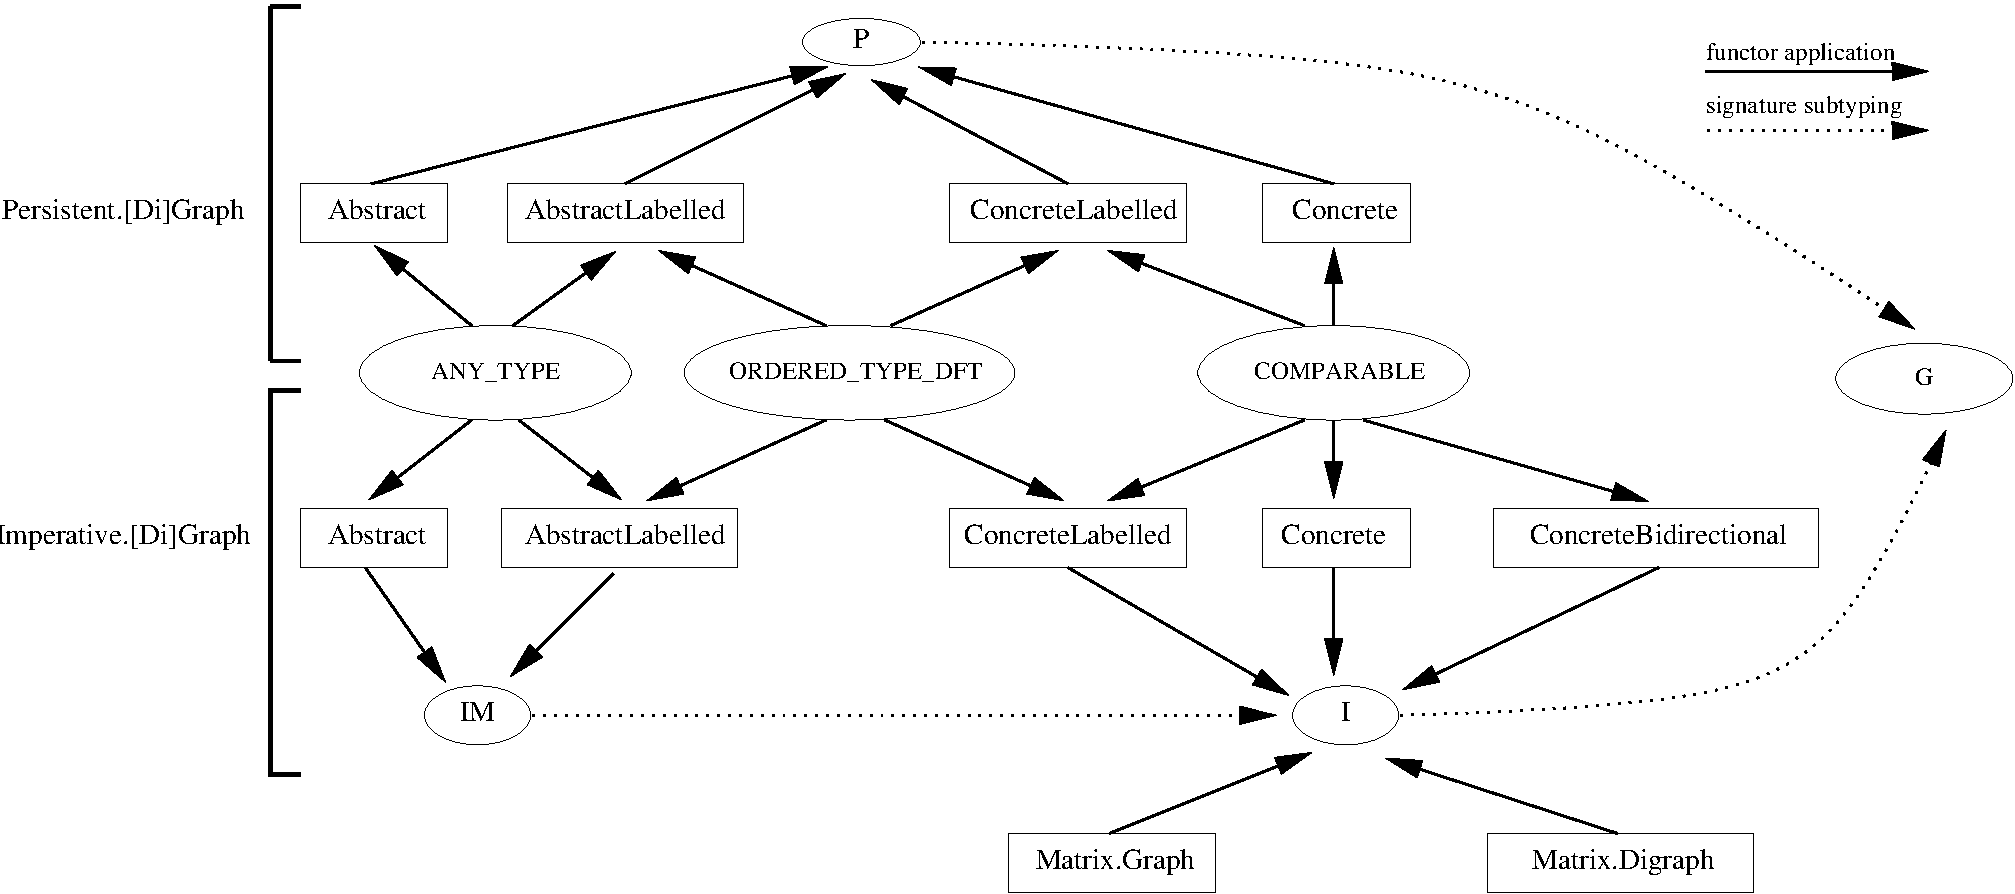
\includegraphics[width=\textwidth]{interface.pdf}    
  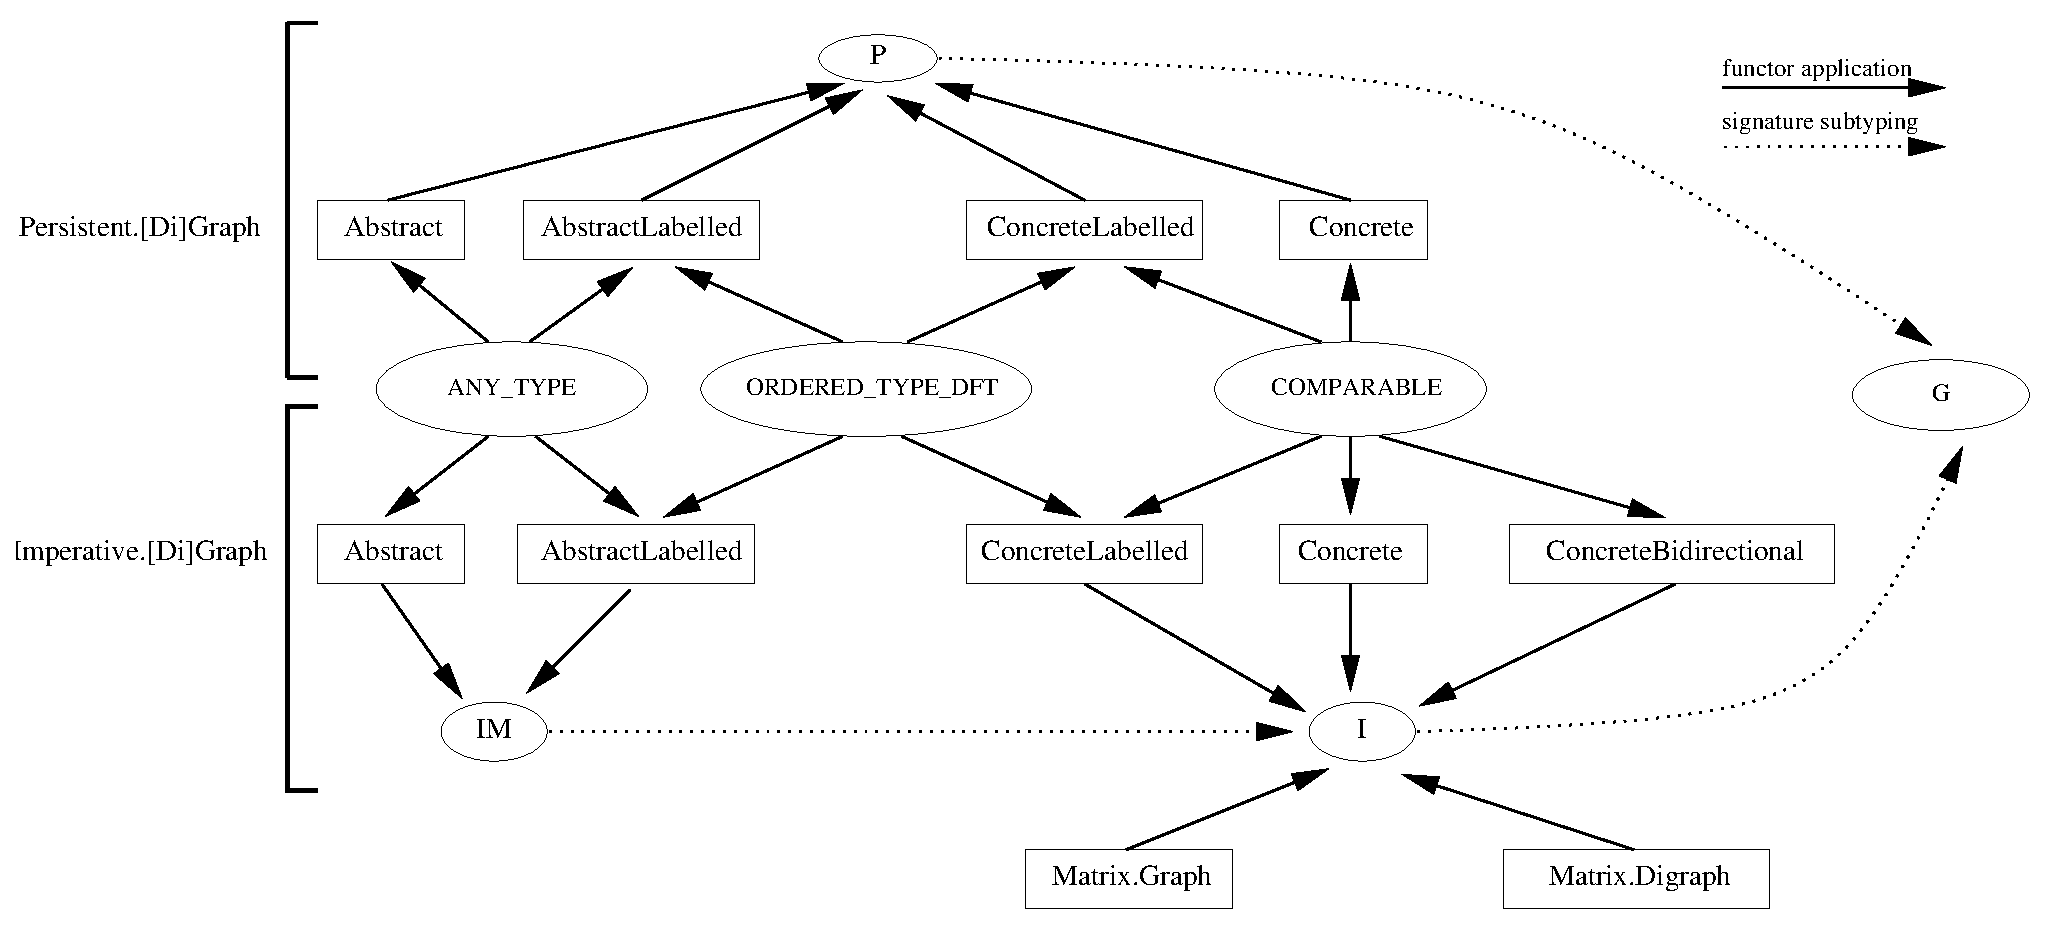
\includegraphics[width=\textwidth]{interface.eps} 
  \caption{\ocamlgraph data structures components}\label{XII:fig:interfaces}
\end{figure*}
Input signatures \texttt{ANY\_TYPE}, \texttt{ORDERED\_TYPE\_DFT} and
\texttt{COMPARABLE} define the user types for vertices and edges
labels. Output signature \texttt{IM} extends signature \texttt{I} with
mutable marks. Three other implementations complete the set of graph
data structures, namely \texttt{ConcreteBidirectional} for graphs with
an efficient access to predecessors, and
\texttt{Matrix.}(\texttt{Graph}, \texttt{Digraph}) for graphs
implemented as adjacency matrices. For efficiency reasons, these three
implementations do not offer the same combination of criteria as the
previous ones.

Several functors are used internally to avoid code duplication among the
functors presented in Figure~\ref{XII:fig:interfaces}. For instance, a
functor adds labels to 
unlabeled graphs; another one encapsulates concrete vertices into an
abstract data type; etc.  Putting it all together, the code size for
the 19 graph data structures is about 1000 lines. This is clearly
small enough to be easily maintained. In Section~\ref{XII:bench} we will
show that this code is also quite efficient.

The graph data structure for our Sudoku solver is simply an imperative
undirected graph with abstract vertices labeled with pairs of integers
and unlabeled edges. It is obtained as:
\begin{alltt}
module G = Imperative.Graph.Abstract
             (struct type t = int \ensuremath{\times} int end) 
\end{alltt}

\section{Generic Algorithms}\label{XII:algos}

This section introduces the second use of functors in \ocamlgraph:
generic programming of graph algorithms.

\subsection{Decoupling Algorithms and Graph Data Structures}

As demonstrated in Section~\ref{XII:implementation}, our library provides
many graph data structures. It makes it necessary to factorize the
code for graph algorithms that operate on these structures. Again,
functors provide a nice encoding of generic algorithms.

The basic idea when coding an algorithm is to focus only on the
required operations that this algorithm imposes on the graph data
structure. Then this algorithm can be expressed naturally as a functor
parameterized by these operations. These operations usually form a
subset of the operations provided by \ocamlgraph graph data
structures. In a few cases, the algorithm requires specific operations
that are independent of the graph data structure. In such a case, the
specific operations are provided as an additional functor parameter.

Such a ``functorization'' of algorithms has two benefits: first, it
allows to add quickly new algorithms to the library, without
duplicating code for all data structures; secondly, it allows the user to
apply an existing algorithm on his own graph data structure.

%% , which is an original feature of \ocamlgraph\ w.r.t. other graph
%% libraries.

\subsection{Example: Depth-First Traversal}
\label{XII:dfs}

We illustrate the generic programming of graph algorithms on the
particular example of depth-first prefix traversal (DFS).  To implement DFS,
we need to iterate over the graph vertices and over the edges leaving
a given vertex. If we do not assume any kind of marks on vertices, we
also need to build a data structure to store the visited nodes. 
We choose a hash table for this purpose and thus we require a hash
function and an equality over vertices.
Thus the minimal input signature for the DFS functor is as follows:
\begin{alltt}
module type G = sig
  type t
  module V : sig
    type t 
    val hash : t \ensuremath{\rightarrow} int 
    val equal : t \ensuremath{\rightarrow} t \ensuremath{\rightarrow} bool 
  end
  val iter_vertex : (V.t \ensuremath{\rightarrow} unit) \ensuremath{\rightarrow} t \ensuremath{\rightarrow} unit
  val iter_succ : (V.t \ensuremath{\rightarrow} unit) \ensuremath{\rightarrow} t \ensuremath{\rightarrow} V.t \ensuremath{\rightarrow} unit
end
\end{alltt}
The DFS algorithm is then implemented as a functor with an argument of
signature \texttt{G}. The result of functor application is a module
providing a single function \texttt{dfs} to traverse a given graph
while applying a given function on all visited vertices:
\begin{alltt}
module Dfs(G : G) : 
  sig val dfs : (G.V.t \ensuremath{\rightarrow} unit) \ensuremath{\rightarrow} G.t \ensuremath{\rightarrow} unit end
\end{alltt}
To implement this functor, we first instantiate \ocaml's generic hash
tables on graph vertices:
\begin{alltt}
module Dfs(G : G) = struct
  module H = Hashtbl.Make(G.V)
\end{alltt}
Then we can implement the traversal. The following code uses a hash
table \texttt{h} to store the vertices already visited and an explicit
stack \texttt{stack} to store the vertices to be visited (to avoid the
possible stack overflow of a recursive implementation). Function
\texttt{G.iter\_vertex} is used to start a DFS on every vertex. The
DFS itself is performed in function \texttt{loop} using \texttt{G.iter\_succ}:
\begin{alltt}
  let dfs f g = 
    let h = H.create 65537 in
    let stack = Stack.create () in
    let push v = 
      if not (H.mem h v) then 
      begin H.add h v (); Stack.push v stack end
    in
    let loop () =
      while not (Stack.is_empty stack) do
        let v = Stack.pop stack in
        f v;
        G.iter_succ push g v
      done
    in
    G.iter_vertex (fun v \ensuremath{\rightarrow} push v; loop ()) g
end
\end{alltt}
Beside this simple algorithm, \ocamlgraph\ provides other kinds of
traversals (breadth-first, postfix, etc.) and more efficient
implementations when the graph data structure contains mutable marks
on vertices.

\subsection{Example: Graph Coloring}
\label{XII:coloring}

As a second example, we present a graph coloring algorithm used in our
Sudoku solver.
For the purpose of our
algorithm, we require the presence of \texttt{get} and \texttt{set}
operations on integer marks associated to vertices. We use these marks
to store the color assigned to each vertex. We also need iterators
over vertices and successors. Thus the minimal signature for a graph
data structure used in our graph coloring algorithm is the following:
\begin{alltt}
module type GM = sig
  type t
  module V : sig type t ... end
  module Mark : sig
    val get : V.t \ensuremath{\rightarrow} int
    val set : V.t \ensuremath{\rightarrow} int \ensuremath{\rightarrow} unit
  end
  val iter_vertex : (V.t \ensuremath{\rightarrow} unit) \ensuremath{\rightarrow} t \ensuremath{\rightarrow} unit
  val iter_succ : (V.t \ensuremath{\rightarrow} unit) \ensuremath{\rightarrow} t \ensuremath{\rightarrow} V.t \ensuremath{\rightarrow} unit
end
\end{alltt}
\ocamlgraph already provides implementations for such a
signature. This is the case for the graph data structure used in our
Sudoku solver.
Then the graph coloring algorithm is implemented as the following functor:
\begin{alltt}
module Coloring(G : GM) : sig
  val coloring : G.t \ensuremath{\rightarrow} int \ensuremath{\rightarrow} unit
end
\end{alltt}
It provides a single function \texttt{coloring} which colors a given
graph with a given number of colors. Some marks may contain initial
constraints. 
% To implement this functor we use a simple backtracking algorithm which
% performs a breadth-first traversal of the graph and successively tries
% each color for each visited vertex. To be able to backtrack during the
% traversal we use persistent cursors~\cite{XII:filliatre06} provided by
% the \texttt{Traverse.Bfs} functor.
% \begin{alltt}
% module Coloring(G : GM) = struct
%   module Bfs = Traverse.Bfs(G)
%
%   let coloring g k =
%     Mark.clear g;
%     let try_color v i =
%       iter_succ 
%         (fun w -> 
%           if Mark.get w = i then raise NoColor) 
%         g v;
%       Mark.set v i
%     in
%     let rec iterate iter =
%       let v = Bfs.get iter in
%       for i = 1 to k do
%         try try_color v i; iterate (Bfs.step iter); 
%             assert false
%         with NoColor -> ()
%       done;
%       Mark.set v 0; raise NoColor
%     in
%     try iterate (Bfs.start g); assert false 
%     with Exit -> ()
% \end{alltt}
To complete our Sudoku solver, we simply need to apply the above
functor on our graph module~\texttt{G}:
\begin{alltt}
module C = Coloring(G)
\end{alltt}
If \texttt{g} contains the Sudoku graph, and
assuming that the initial constraints are set in \texttt{g} marks, 
solving the Sudoku amounts to 9-coloring graph \texttt{g}:
\begin{alltt}
C.coloring g 9
\end{alltt}


\subsection{Building Graphs}\label{XII:builder}

In Section~\ref{XII:interface}, we have shown that persistent and
imperative graphs have creation functions with different signatures.
However, as we have written algorithms in a generic way, we may want
to build graphs in a generic way, that is independently of the
underlying data structure. For instance, we may want to implement
graph operations (such as union, transitive closure, etc.) or to build
some classic graphs (such as the full graph with $n$ vertices, the de
Bruijn graph of order $n$, etc.) or even random graphs. In all these
cases, the persistent or imperative nature of the graph is not really
significant but the signature difference disallows genericity.

To solve this issue, we introduce a module \texttt{Builder}. It
defines a common interface for graphs building:
\begin{alltt}
module type S = sig
  module G : Sig.G
  val empty : unit \fl G.t
  val copy : G.t \fl G.t
  val add_vertex : G.t \fl G.V.t \fl G.t
  val add_edge : G.t \fl G.V.t \fl G.V.t \fl G.t
  val add_edge_e : G.t \fl G.E.t \fl G.t
end
\end{alltt}
It is immediate to realize such a signature for persistent or
imperative graphs:
\begin{alltt}
module P(G : Sig.P) : S with module G = G
module I(G : Sig.I) : S with module G = G
\end{alltt}
It is important to notice that for imperative graphs the values
returned by the functions \texttt{add\_vertex},
\texttt{add\_edge} and \texttt{add\_edge\_e} are meaningless.

Therefore, it is easy to write a generic algorithm that builds graphs.
First we write a generic version as a functor taking a module of
signature \texttt{Builder.S} as argument:
\begin{alltt}
module Make(B : Builder.S) = struct ... end
\end{alltt}
and then we can trivially provide two variants of this functor for
both persistent and imperative graphs, with the following two lines:
\begin{alltt}
module P(G : Sig.P) = Make(Builder.P(G))
module I(G : Sig.I) = Make(Builder.I(G))
\end{alltt}
Thus the use of the module \texttt{Builder} is entirely hidden from
the user point of view.


\section{Benchmarks}\label{XII:bench}

Surprisingly, we could not find any standard benchmark for graph
libraries. In order to give an idea of \ocamlgraph efficiency, we
present here the results of a little benchmark of our own.  We test
four different data structures for undirected graphs with unlabeled
edges, that are either persistent (P) or imperative (I) and with
either abstract (A) or concrete (C) vertices. In the following, these
are referred to as PA, PC, IA and IC, respectively.  All tests were
performed on a Pentium 4 2.4 GHz.

We first test the efficiency of graph creation and mutation.  For that
purpose, we build cliques of $V$ vertices (and thus $E=V(V+1)/2$
edges since we include self loops).  Then we repeatedly delete all
edges and vertices in these graphs.  Figure~\ref{XII:fig:bench:build}
displays the creation and deletion timings in seconds up to $V=1000$
(that is half a million edges).  The speed of creation observed is
roughly 100,000 edges per second for imperative graphs. The creation
of persistent graphs is slower but within a constant factor (less than
2). Deletion is twice as fast as creation.  Regarding memory
consumption, all four data structures use approximately 5 machine words
(typically 20 bytes) per edge.

\begin{figure*}
  \centering%\hspace*{-2em}
  % GNUPLOT: LaTeX picture
\setlength{\unitlength}{0.240900pt}
\ifx\plotpoint\undefined\newsavebox{\plotpoint}\fi
\sbox{\plotpoint}{\rule[-0.200pt]{0.400pt}{0.400pt}}%
\begin{picture}(1049,629)(0,0)
\sbox{\plotpoint}{\rule[-0.200pt]{0.400pt}{0.400pt}}%
\put(120.0,123.0){\rule[-0.200pt]{4.818pt}{0.400pt}}
\put(100,123){\makebox(0,0)[r]{ 0}}
\put(969.0,123.0){\rule[-0.200pt]{4.818pt}{0.400pt}}
\put(120.0,170.0){\rule[-0.200pt]{4.818pt}{0.400pt}}
\put(100,170){\makebox(0,0)[r]{ 2}}
\put(969.0,170.0){\rule[-0.200pt]{4.818pt}{0.400pt}}
\put(120.0,216.0){\rule[-0.200pt]{4.818pt}{0.400pt}}
\put(100,216){\makebox(0,0)[r]{ 4}}
\put(969.0,216.0){\rule[-0.200pt]{4.818pt}{0.400pt}}
\put(120.0,263.0){\rule[-0.200pt]{4.818pt}{0.400pt}}
\put(100,263){\makebox(0,0)[r]{ 6}}
\put(969.0,263.0){\rule[-0.200pt]{4.818pt}{0.400pt}}
\put(120.0,310.0){\rule[-0.200pt]{4.818pt}{0.400pt}}
\put(100,310){\makebox(0,0)[r]{ 8}}
\put(969.0,310.0){\rule[-0.200pt]{4.818pt}{0.400pt}}
\put(120.0,357.0){\rule[-0.200pt]{4.818pt}{0.400pt}}
\put(100,357){\makebox(0,0)[r]{ 10}}
\put(969.0,357.0){\rule[-0.200pt]{4.818pt}{0.400pt}}
\put(120.0,403.0){\rule[-0.200pt]{4.818pt}{0.400pt}}
\put(100,403){\makebox(0,0)[r]{ 12}}
\put(969.0,403.0){\rule[-0.200pt]{4.818pt}{0.400pt}}
\put(120.0,450.0){\rule[-0.200pt]{4.818pt}{0.400pt}}
\put(100,450){\makebox(0,0)[r]{ 14}}
\put(969.0,450.0){\rule[-0.200pt]{4.818pt}{0.400pt}}
\put(120.0,497.0){\rule[-0.200pt]{4.818pt}{0.400pt}}
\put(100,497){\makebox(0,0)[r]{ 16}}
\put(969.0,497.0){\rule[-0.200pt]{4.818pt}{0.400pt}}
\put(120.0,543.0){\rule[-0.200pt]{4.818pt}{0.400pt}}
\put(100,543){\makebox(0,0)[r]{ 18}}
\put(969.0,543.0){\rule[-0.200pt]{4.818pt}{0.400pt}}
\put(120.0,590.0){\rule[-0.200pt]{4.818pt}{0.400pt}}
\put(100,590){\makebox(0,0)[r]{ 20}}
\put(969.0,590.0){\rule[-0.200pt]{4.818pt}{0.400pt}}
\put(120.0,123.0){\rule[-0.200pt]{0.400pt}{4.818pt}}
\put(120,82){\makebox(0,0){ 100}}
\put(120.0,570.0){\rule[-0.200pt]{0.400pt}{4.818pt}}
\put(217.0,123.0){\rule[-0.200pt]{0.400pt}{4.818pt}}
\put(217,82){\makebox(0,0){ 200}}
\put(217.0,570.0){\rule[-0.200pt]{0.400pt}{4.818pt}}
\put(313.0,123.0){\rule[-0.200pt]{0.400pt}{4.818pt}}
\put(313,82){\makebox(0,0){ 300}}
\put(313.0,570.0){\rule[-0.200pt]{0.400pt}{4.818pt}}
\put(410.0,123.0){\rule[-0.200pt]{0.400pt}{4.818pt}}
\put(410,82){\makebox(0,0){ 400}}
\put(410.0,570.0){\rule[-0.200pt]{0.400pt}{4.818pt}}
\put(506.0,123.0){\rule[-0.200pt]{0.400pt}{4.818pt}}
\put(506,82){\makebox(0,0){ 500}}
\put(506.0,570.0){\rule[-0.200pt]{0.400pt}{4.818pt}}
\put(603.0,123.0){\rule[-0.200pt]{0.400pt}{4.818pt}}
\put(603,82){\makebox(0,0){ 600}}
\put(603.0,570.0){\rule[-0.200pt]{0.400pt}{4.818pt}}
\put(699.0,123.0){\rule[-0.200pt]{0.400pt}{4.818pt}}
\put(699,82){\makebox(0,0){ 700}}
\put(699.0,570.0){\rule[-0.200pt]{0.400pt}{4.818pt}}
\put(796.0,123.0){\rule[-0.200pt]{0.400pt}{4.818pt}}
\put(796,82){\makebox(0,0){ 800}}
\put(796.0,570.0){\rule[-0.200pt]{0.400pt}{4.818pt}}
\put(892.0,123.0){\rule[-0.200pt]{0.400pt}{4.818pt}}
\put(892,82){\makebox(0,0){ 900}}
\put(892.0,570.0){\rule[-0.200pt]{0.400pt}{4.818pt}}
\put(989.0,123.0){\rule[-0.200pt]{0.400pt}{4.818pt}}
\put(989,82){\makebox(0,0){ 1000}}
\put(989.0,570.0){\rule[-0.200pt]{0.400pt}{4.818pt}}
\put(120.0,123.0){\rule[-0.200pt]{209.342pt}{0.400pt}}
\put(989.0,123.0){\rule[-0.200pt]{0.400pt}{112.500pt}}
\put(120.0,590.0){\rule[-0.200pt]{209.342pt}{0.400pt}}
\put(120.0,123.0){\rule[-0.200pt]{0.400pt}{112.500pt}}
\put(554,21){\makebox(0,0){number of nodes $V$}}
\put(180,550){\makebox(0,0)[r]{IA}}
\put(200.0,550.0){\rule[-0.200pt]{24.090pt}{0.400pt}}
\put(120,124){\usebox{\plotpoint}}
\multiput(120.00,124.60)(14.080,0.468){5}{\rule{9.800pt}{0.113pt}}
\multiput(120.00,123.17)(76.660,4.000){2}{\rule{4.900pt}{0.400pt}}
\multiput(217.00,128.58)(4.505,0.492){19}{\rule{3.591pt}{0.118pt}}
\multiput(217.00,127.17)(88.547,11.000){2}{\rule{1.795pt}{0.400pt}}
\multiput(313.00,139.58)(2.739,0.495){33}{\rule{2.256pt}{0.119pt}}
\multiput(313.00,138.17)(92.318,18.000){2}{\rule{1.128pt}{0.400pt}}
\multiput(410.00,157.58)(1.939,0.497){47}{\rule{1.636pt}{0.120pt}}
\multiput(410.00,156.17)(92.604,25.000){2}{\rule{0.818pt}{0.400pt}}
\multiput(506.00,182.58)(1.479,0.497){63}{\rule{1.276pt}{0.120pt}}
\multiput(506.00,181.17)(94.352,33.000){2}{\rule{0.638pt}{0.400pt}}
\multiput(603.00,215.58)(2.111,0.496){43}{\rule{1.770pt}{0.120pt}}
\multiput(603.00,214.17)(92.327,23.000){2}{\rule{0.885pt}{0.400pt}}
\multiput(699.00,238.58)(1.188,0.498){79}{\rule{1.046pt}{0.120pt}}
\multiput(699.00,237.17)(94.828,41.000){2}{\rule{0.523pt}{0.400pt}}
\multiput(796.00,279.58)(0.801,0.499){117}{\rule{0.740pt}{0.120pt}}
\multiput(796.00,278.17)(94.464,60.000){2}{\rule{0.370pt}{0.400pt}}
\multiput(892.00,339.58)(1.249,0.498){75}{\rule{1.095pt}{0.120pt}}
\multiput(892.00,338.17)(94.728,39.000){2}{\rule{0.547pt}{0.400pt}}
\put(180,509){\makebox(0,0)[r]{IC}}
\multiput(200,509)(20.756,0.000){5}{\usebox{\plotpoint}}
\put(300,509){\usebox{\plotpoint}}
\put(120,124){\usebox{\plotpoint}}
\multiput(120,124)(20.685,1.706){5}{\usebox{\plotpoint}}
\multiput(217,132)(20.665,1.937){5}{\usebox{\plotpoint}}
\multiput(313,141)(20.368,3.990){5}{\usebox{\plotpoint}}
\multiput(410,160)(20.086,5.231){4}{\usebox{\plotpoint}}
\multiput(506,185)(20.572,2.757){5}{\usebox{\plotpoint}}
\multiput(603,198)(18.564,9.282){5}{\usebox{\plotpoint}}
\multiput(699,246)(18.293,9.806){6}{\usebox{\plotpoint}}
\multiput(796,298)(19.299,7.639){5}{\usebox{\plotpoint}}
\multiput(892,336)(18.135,10.096){5}{\usebox{\plotpoint}}
\put(989,390){\usebox{\plotpoint}}
\sbox{\plotpoint}{\rule[-0.400pt]{0.800pt}{0.800pt}}%
\sbox{\plotpoint}{\rule[-0.200pt]{0.400pt}{0.400pt}}%
\put(180,468){\makebox(0,0)[r]{PA}}
\sbox{\plotpoint}{\rule[-0.400pt]{0.800pt}{0.800pt}}%
\put(200.0,468.0){\rule[-0.400pt]{24.090pt}{0.800pt}}
\put(120,124){\usebox{\plotpoint}}
\multiput(120.00,125.40)(5.330,0.514){13}{\rule{7.960pt}{0.124pt}}
\multiput(120.00,122.34)(80.479,10.000){2}{\rule{3.980pt}{0.800pt}}
\multiput(217.00,135.40)(5.975,0.516){11}{\rule{8.733pt}{0.124pt}}
\multiput(217.00,132.34)(77.874,9.000){2}{\rule{4.367pt}{0.800pt}}
\multiput(313.00,144.41)(2.377,0.505){35}{\rule{3.895pt}{0.122pt}}
\multiput(313.00,141.34)(88.915,21.000){2}{\rule{1.948pt}{0.800pt}}
\multiput(410.00,165.41)(1.311,0.503){67}{\rule{2.276pt}{0.121pt}}
\multiput(410.00,162.34)(91.277,37.000){2}{\rule{1.138pt}{0.800pt}}
\multiput(506.00,202.41)(0.996,0.502){91}{\rule{1.784pt}{0.121pt}}
\multiput(506.00,199.34)(93.298,49.000){2}{\rule{0.892pt}{0.800pt}}
\multiput(603.00,251.41)(1.311,0.503){67}{\rule{2.276pt}{0.121pt}}
\multiput(603.00,248.34)(91.277,37.000){2}{\rule{1.138pt}{0.800pt}}
\multiput(699.00,288.41)(0.854,0.502){107}{\rule{1.561pt}{0.121pt}}
\multiput(699.00,285.34)(93.759,57.000){2}{\rule{0.781pt}{0.800pt}}
\multiput(796.00,345.41)(0.640,0.501){143}{\rule{1.224pt}{0.121pt}}
\multiput(796.00,342.34)(93.460,75.000){2}{\rule{0.612pt}{0.800pt}}
\multiput(892.00,420.41)(0.614,0.501){151}{\rule{1.182pt}{0.121pt}}
\multiput(892.00,417.34)(94.546,79.000){2}{\rule{0.591pt}{0.800pt}}
\sbox{\plotpoint}{\rule[-0.500pt]{1.000pt}{1.000pt}}%
\sbox{\plotpoint}{\rule[-0.200pt]{0.400pt}{0.400pt}}%
\put(180,427){\makebox(0,0)[r]{PC}}
\sbox{\plotpoint}{\rule[-0.500pt]{1.000pt}{1.000pt}}%
\multiput(200,427)(20.756,0.000){5}{\usebox{\plotpoint}}
\put(300,427){\usebox{\plotpoint}}
\put(120,125){\usebox{\plotpoint}}
\multiput(120,125)(20.598,2.548){5}{\usebox{\plotpoint}}
\multiput(217,137)(20.595,2.574){5}{\usebox{\plotpoint}}
\multiput(313,149)(19.941,5.756){5}{\usebox{\plotpoint}}
\multiput(410,177)(18.718,8.969){5}{\usebox{\plotpoint}}
\multiput(506,223)(17.652,10.918){5}{\usebox{\plotpoint}}
\multiput(603,283)(18.793,8.809){5}{\usebox{\plotpoint}}
\multiput(699,328)(15.215,14.117){7}{\usebox{\plotpoint}}
\multiput(796,418)(16.771,12.229){6}{\usebox{\plotpoint}}
\multiput(892,488)(14.377,14.970){6}{\usebox{\plotpoint}}
\put(989,589){\usebox{\plotpoint}}
\sbox{\plotpoint}{\rule[-0.200pt]{0.400pt}{0.400pt}}%
\put(120.0,123.0){\rule[-0.200pt]{209.342pt}{0.400pt}}
\put(989.0,123.0){\rule[-0.200pt]{0.400pt}{112.500pt}}
\put(120.0,590.0){\rule[-0.200pt]{209.342pt}{0.400pt}}
\put(120.0,123.0){\rule[-0.200pt]{0.400pt}{112.500pt}}
\end{picture}


  % GNUPLOT: LaTeX picture
\setlength{\unitlength}{0.240900pt}
\ifx\plotpoint\undefined\newsavebox{\plotpoint}\fi
\begin{picture}(1049,629)(0,0)
\sbox{\plotpoint}{\rule[-0.200pt]{0.400pt}{0.400pt}}%
\put(100.0,123.0){\rule[-0.200pt]{4.818pt}{0.400pt}}
\put(80,123){\makebox(0,0)[r]{ 0}}
\put(969.0,123.0){\rule[-0.200pt]{4.818pt}{0.400pt}}
\put(100.0,175.0){\rule[-0.200pt]{4.818pt}{0.400pt}}
\put(80,175){\makebox(0,0)[r]{ 1}}
\put(969.0,175.0){\rule[-0.200pt]{4.818pt}{0.400pt}}
\put(100.0,227.0){\rule[-0.200pt]{4.818pt}{0.400pt}}
\put(80,227){\makebox(0,0)[r]{ 2}}
\put(969.0,227.0){\rule[-0.200pt]{4.818pt}{0.400pt}}
\put(100.0,279.0){\rule[-0.200pt]{4.818pt}{0.400pt}}
\put(80,279){\makebox(0,0)[r]{ 3}}
\put(969.0,279.0){\rule[-0.200pt]{4.818pt}{0.400pt}}
\put(100.0,331.0){\rule[-0.200pt]{4.818pt}{0.400pt}}
\put(80,331){\makebox(0,0)[r]{ 4}}
\put(969.0,331.0){\rule[-0.200pt]{4.818pt}{0.400pt}}
\put(100.0,382.0){\rule[-0.200pt]{4.818pt}{0.400pt}}
\put(80,382){\makebox(0,0)[r]{ 5}}
\put(969.0,382.0){\rule[-0.200pt]{4.818pt}{0.400pt}}
\put(100.0,434.0){\rule[-0.200pt]{4.818pt}{0.400pt}}
\put(80,434){\makebox(0,0)[r]{ 6}}
\put(969.0,434.0){\rule[-0.200pt]{4.818pt}{0.400pt}}
\put(100.0,486.0){\rule[-0.200pt]{4.818pt}{0.400pt}}
\put(80,486){\makebox(0,0)[r]{ 7}}
\put(969.0,486.0){\rule[-0.200pt]{4.818pt}{0.400pt}}
\put(100.0,538.0){\rule[-0.200pt]{4.818pt}{0.400pt}}
\put(80,538){\makebox(0,0)[r]{ 8}}
\put(969.0,538.0){\rule[-0.200pt]{4.818pt}{0.400pt}}
\put(100.0,590.0){\rule[-0.200pt]{4.818pt}{0.400pt}}
\put(80,590){\makebox(0,0)[r]{ 9}}
\put(969.0,590.0){\rule[-0.200pt]{4.818pt}{0.400pt}}
\put(100.0,123.0){\rule[-0.200pt]{0.400pt}{4.818pt}}
\put(100,82){\makebox(0,0){ 100}}
\put(100.0,570.0){\rule[-0.200pt]{0.400pt}{4.818pt}}
\put(199.0,123.0){\rule[-0.200pt]{0.400pt}{4.818pt}}
\put(199,82){\makebox(0,0){ 200}}
\put(199.0,570.0){\rule[-0.200pt]{0.400pt}{4.818pt}}
\put(298.0,123.0){\rule[-0.200pt]{0.400pt}{4.818pt}}
\put(298,82){\makebox(0,0){ 300}}
\put(298.0,570.0){\rule[-0.200pt]{0.400pt}{4.818pt}}
\put(396.0,123.0){\rule[-0.200pt]{0.400pt}{4.818pt}}
\put(396,82){\makebox(0,0){ 400}}
\put(396.0,570.0){\rule[-0.200pt]{0.400pt}{4.818pt}}
\put(495.0,123.0){\rule[-0.200pt]{0.400pt}{4.818pt}}
\put(495,82){\makebox(0,0){ 500}}
\put(495.0,570.0){\rule[-0.200pt]{0.400pt}{4.818pt}}
\put(594.0,123.0){\rule[-0.200pt]{0.400pt}{4.818pt}}
\put(594,82){\makebox(0,0){ 600}}
\put(594.0,570.0){\rule[-0.200pt]{0.400pt}{4.818pt}}
\put(693.0,123.0){\rule[-0.200pt]{0.400pt}{4.818pt}}
\put(693,82){\makebox(0,0){ 700}}
\put(693.0,570.0){\rule[-0.200pt]{0.400pt}{4.818pt}}
\put(791.0,123.0){\rule[-0.200pt]{0.400pt}{4.818pt}}
\put(791,82){\makebox(0,0){ 800}}
\put(791.0,570.0){\rule[-0.200pt]{0.400pt}{4.818pt}}
\put(890.0,123.0){\rule[-0.200pt]{0.400pt}{4.818pt}}
\put(890,82){\makebox(0,0){ 900}}
\put(890.0,570.0){\rule[-0.200pt]{0.400pt}{4.818pt}}
\put(989.0,123.0){\rule[-0.200pt]{0.400pt}{4.818pt}}
\put(989,82){\makebox(0,0){ 1000}}
\put(989.0,570.0){\rule[-0.200pt]{0.400pt}{4.818pt}}
\put(100.0,123.0){\rule[-0.200pt]{214.160pt}{0.400pt}}
\put(989.0,123.0){\rule[-0.200pt]{0.400pt}{112.500pt}}
\put(100.0,590.0){\rule[-0.200pt]{214.160pt}{0.400pt}}
\put(100.0,123.0){\rule[-0.200pt]{0.400pt}{112.500pt}}
\put(544,21){\makebox(0,0){number of nodes $V$}}
\put(160,550){\makebox(0,0)[r]{IA}}
\put(180.0,550.0){\rule[-0.200pt]{24.090pt}{0.400pt}}
\put(100,124){\usebox{\plotpoint}}
\multiput(100.00,124.61)(21.895,0.447){3}{\rule{13.300pt}{0.108pt}}
\multiput(100.00,123.17)(71.395,3.000){2}{\rule{6.650pt}{0.400pt}}
\multiput(199.00,127.59)(8.898,0.482){9}{\rule{6.700pt}{0.116pt}}
\multiput(199.00,126.17)(85.094,6.000){2}{\rule{3.350pt}{0.400pt}}
\multiput(298.00,133.58)(4.600,0.492){19}{\rule{3.664pt}{0.118pt}}
\multiput(298.00,132.17)(90.396,11.000){2}{\rule{1.832pt}{0.400pt}}
\multiput(396.00,144.58)(2.964,0.495){31}{\rule{2.429pt}{0.119pt}}
\multiput(396.00,143.17)(93.958,17.000){2}{\rule{1.215pt}{0.400pt}}
\multiput(495.00,161.58)(3.370,0.494){27}{\rule{2.740pt}{0.119pt}}
\multiput(495.00,160.17)(93.313,15.000){2}{\rule{1.370pt}{0.400pt}}
\multiput(594.00,176.58)(0.739,0.499){131}{\rule{0.691pt}{0.120pt}}
\multiput(594.00,175.17)(97.566,67.000){2}{\rule{0.346pt}{0.400pt}}
\multiput(693.00,241.92)(3.867,-0.493){23}{\rule{3.115pt}{0.119pt}}
\multiput(693.00,242.17)(91.534,-13.000){2}{\rule{1.558pt}{0.400pt}}
\multiput(791.58,230.00)(0.499,0.576){195}{\rule{0.120pt}{0.561pt}}
\multiput(790.17,230.00)(99.000,112.836){2}{\rule{0.400pt}{0.280pt}}
\multiput(890.00,344.58)(1.156,0.498){83}{\rule{1.021pt}{0.120pt}}
\multiput(890.00,343.17)(96.881,43.000){2}{\rule{0.510pt}{0.400pt}}
\put(160,509){\makebox(0,0)[r]{IC}}
\multiput(180,509)(20.756,0.000){5}{\usebox{\plotpoint}}
\put(280,509){\usebox{\plotpoint}}
\put(100,124){\usebox{\plotpoint}}
\multiput(100,124)(20.739,0.838){5}{\usebox{\plotpoint}}
\multiput(199,128)(20.717,1.256){5}{\usebox{\plotpoint}}
\multiput(298,134)(20.602,2.523){5}{\usebox{\plotpoint}}
\multiput(396,146)(20.754,0.210){5}{\usebox{\plotpoint}}
\multiput(495,147)(17.350,11.391){5}{\usebox{\plotpoint}}
\multiput(594,212)(20.751,-0.419){5}{\usebox{\plotpoint}}
\multiput(693,210)(15.918,13.319){6}{\usebox{\plotpoint}}
\multiput(791,292)(18.750,8.901){5}{\usebox{\plotpoint}}
\multiput(890,339)(17.028,11.868){6}{\usebox{\plotpoint}}
\put(989,408){\usebox{\plotpoint}}
\sbox{\plotpoint}{\rule[-0.400pt]{0.800pt}{0.800pt}}%
\sbox{\plotpoint}{\rule[-0.200pt]{0.400pt}{0.400pt}}%
\put(160,468){\makebox(0,0)[r]{PA}}
\sbox{\plotpoint}{\rule[-0.400pt]{0.800pt}{0.800pt}}%
\put(180.0,468.0){\rule[-0.400pt]{24.090pt}{0.800pt}}
\put(100,125){\usebox{\plotpoint}}
\multiput(100.00,126.40)(8.534,0.526){7}{\rule{11.514pt}{0.127pt}}
\multiput(100.00,123.34)(75.102,7.000){2}{\rule{5.757pt}{0.800pt}}
\multiput(199.00,133.41)(3.032,0.507){27}{\rule{4.859pt}{0.122pt}}
\multiput(199.00,130.34)(88.915,17.000){2}{\rule{2.429pt}{0.800pt}}
\multiput(298.00,150.41)(4.378,0.511){17}{\rule{6.733pt}{0.123pt}}
\multiput(298.00,147.34)(84.025,12.000){2}{\rule{3.367pt}{0.800pt}}
\multiput(396.00,162.41)(1.801,0.504){49}{\rule{3.029pt}{0.121pt}}
\multiput(396.00,159.34)(92.714,28.000){2}{\rule{1.514pt}{0.800pt}}
\multiput(495.00,190.41)(0.828,0.502){113}{\rule{1.520pt}{0.121pt}}
\multiput(495.00,187.34)(95.845,60.000){2}{\rule{0.760pt}{0.800pt}}
\multiput(594.00,250.41)(1.084,0.502){85}{\rule{1.922pt}{0.121pt}}
\multiput(594.00,247.34)(95.011,46.000){2}{\rule{0.961pt}{0.800pt}}
\multiput(693.00,296.41)(0.819,0.502){113}{\rule{1.507pt}{0.121pt}}
\multiput(693.00,293.34)(94.873,60.000){2}{\rule{0.753pt}{0.800pt}}
\multiput(791.00,356.41)(0.688,0.501){137}{\rule{1.300pt}{0.121pt}}
\multiput(791.00,353.34)(96.302,72.000){2}{\rule{0.650pt}{0.800pt}}
\multiput(890.00,428.41)(0.669,0.501){141}{\rule{1.270pt}{0.121pt}}
\multiput(890.00,425.34)(96.363,74.000){2}{\rule{0.635pt}{0.800pt}}
\sbox{\plotpoint}{\rule[-0.500pt]{1.000pt}{1.000pt}}%
\sbox{\plotpoint}{\rule[-0.200pt]{0.400pt}{0.400pt}}%
\put(160,427){\makebox(0,0)[r]{PC}}
\sbox{\plotpoint}{\rule[-0.500pt]{1.000pt}{1.000pt}}%
\multiput(180,427)(20.756,0.000){5}{\usebox{\plotpoint}}
\put(280,427){\usebox{\plotpoint}}
\put(100,125){\usebox{\plotpoint}}
\multiput(100,125)(20.704,1.464){5}{\usebox{\plotpoint}}
\multiput(199,132)(20.171,4.890){5}{\usebox{\plotpoint}}
\multiput(298,156)(20.414,3.750){5}{\usebox{\plotpoint}}
\multiput(396,174)(19.569,6.918){5}{\usebox{\plotpoint}}
\multiput(495,209)(17.350,11.391){6}{\usebox{\plotpoint}}
\multiput(594,274)(20.261,4.503){5}{\usebox{\plotpoint}}
\multiput(693,296)(13.599,15.680){7}{\usebox{\plotpoint}}
\multiput(791,409)(15.435,13.876){6}{\usebox{\plotpoint}}
\multiput(890,498)(15.984,13.240){6}{\usebox{\plotpoint}}
\put(989,580){\usebox{\plotpoint}}
\sbox{\plotpoint}{\rule[-0.200pt]{0.400pt}{0.400pt}}%
\put(100.0,123.0){\rule[-0.200pt]{214.160pt}{0.400pt}}
\put(989.0,123.0){\rule[-0.200pt]{0.400pt}{112.500pt}}
\put(100.0,590.0){\rule[-0.200pt]{214.160pt}{0.400pt}}
\put(100.0,123.0){\rule[-0.200pt]{0.400pt}{112.500pt}}
\end{picture}

%%   \begin{tabular}{cc}
%%   \begin{minipage}{0.5\linewidth}
%%     % GNUPLOT: LaTeX picture
\setlength{\unitlength}{0.240900pt}
\ifx\plotpoint\undefined\newsavebox{\plotpoint}\fi
\sbox{\plotpoint}{\rule[-0.200pt]{0.400pt}{0.400pt}}%
\begin{picture}(1049,629)(0,0)
\sbox{\plotpoint}{\rule[-0.200pt]{0.400pt}{0.400pt}}%
\put(120.0,123.0){\rule[-0.200pt]{4.818pt}{0.400pt}}
\put(100,123){\makebox(0,0)[r]{ 0}}
\put(969.0,123.0){\rule[-0.200pt]{4.818pt}{0.400pt}}
\put(120.0,170.0){\rule[-0.200pt]{4.818pt}{0.400pt}}
\put(100,170){\makebox(0,0)[r]{ 2}}
\put(969.0,170.0){\rule[-0.200pt]{4.818pt}{0.400pt}}
\put(120.0,216.0){\rule[-0.200pt]{4.818pt}{0.400pt}}
\put(100,216){\makebox(0,0)[r]{ 4}}
\put(969.0,216.0){\rule[-0.200pt]{4.818pt}{0.400pt}}
\put(120.0,263.0){\rule[-0.200pt]{4.818pt}{0.400pt}}
\put(100,263){\makebox(0,0)[r]{ 6}}
\put(969.0,263.0){\rule[-0.200pt]{4.818pt}{0.400pt}}
\put(120.0,310.0){\rule[-0.200pt]{4.818pt}{0.400pt}}
\put(100,310){\makebox(0,0)[r]{ 8}}
\put(969.0,310.0){\rule[-0.200pt]{4.818pt}{0.400pt}}
\put(120.0,357.0){\rule[-0.200pt]{4.818pt}{0.400pt}}
\put(100,357){\makebox(0,0)[r]{ 10}}
\put(969.0,357.0){\rule[-0.200pt]{4.818pt}{0.400pt}}
\put(120.0,403.0){\rule[-0.200pt]{4.818pt}{0.400pt}}
\put(100,403){\makebox(0,0)[r]{ 12}}
\put(969.0,403.0){\rule[-0.200pt]{4.818pt}{0.400pt}}
\put(120.0,450.0){\rule[-0.200pt]{4.818pt}{0.400pt}}
\put(100,450){\makebox(0,0)[r]{ 14}}
\put(969.0,450.0){\rule[-0.200pt]{4.818pt}{0.400pt}}
\put(120.0,497.0){\rule[-0.200pt]{4.818pt}{0.400pt}}
\put(100,497){\makebox(0,0)[r]{ 16}}
\put(969.0,497.0){\rule[-0.200pt]{4.818pt}{0.400pt}}
\put(120.0,543.0){\rule[-0.200pt]{4.818pt}{0.400pt}}
\put(100,543){\makebox(0,0)[r]{ 18}}
\put(969.0,543.0){\rule[-0.200pt]{4.818pt}{0.400pt}}
\put(120.0,590.0){\rule[-0.200pt]{4.818pt}{0.400pt}}
\put(100,590){\makebox(0,0)[r]{ 20}}
\put(969.0,590.0){\rule[-0.200pt]{4.818pt}{0.400pt}}
\put(120.0,123.0){\rule[-0.200pt]{0.400pt}{4.818pt}}
\put(120,82){\makebox(0,0){ 100}}
\put(120.0,570.0){\rule[-0.200pt]{0.400pt}{4.818pt}}
\put(217.0,123.0){\rule[-0.200pt]{0.400pt}{4.818pt}}
\put(217,82){\makebox(0,0){ 200}}
\put(217.0,570.0){\rule[-0.200pt]{0.400pt}{4.818pt}}
\put(313.0,123.0){\rule[-0.200pt]{0.400pt}{4.818pt}}
\put(313,82){\makebox(0,0){ 300}}
\put(313.0,570.0){\rule[-0.200pt]{0.400pt}{4.818pt}}
\put(410.0,123.0){\rule[-0.200pt]{0.400pt}{4.818pt}}
\put(410,82){\makebox(0,0){ 400}}
\put(410.0,570.0){\rule[-0.200pt]{0.400pt}{4.818pt}}
\put(506.0,123.0){\rule[-0.200pt]{0.400pt}{4.818pt}}
\put(506,82){\makebox(0,0){ 500}}
\put(506.0,570.0){\rule[-0.200pt]{0.400pt}{4.818pt}}
\put(603.0,123.0){\rule[-0.200pt]{0.400pt}{4.818pt}}
\put(603,82){\makebox(0,0){ 600}}
\put(603.0,570.0){\rule[-0.200pt]{0.400pt}{4.818pt}}
\put(699.0,123.0){\rule[-0.200pt]{0.400pt}{4.818pt}}
\put(699,82){\makebox(0,0){ 700}}
\put(699.0,570.0){\rule[-0.200pt]{0.400pt}{4.818pt}}
\put(796.0,123.0){\rule[-0.200pt]{0.400pt}{4.818pt}}
\put(796,82){\makebox(0,0){ 800}}
\put(796.0,570.0){\rule[-0.200pt]{0.400pt}{4.818pt}}
\put(892.0,123.0){\rule[-0.200pt]{0.400pt}{4.818pt}}
\put(892,82){\makebox(0,0){ 900}}
\put(892.0,570.0){\rule[-0.200pt]{0.400pt}{4.818pt}}
\put(989.0,123.0){\rule[-0.200pt]{0.400pt}{4.818pt}}
\put(989,82){\makebox(0,0){ 1000}}
\put(989.0,570.0){\rule[-0.200pt]{0.400pt}{4.818pt}}
\put(120.0,123.0){\rule[-0.200pt]{209.342pt}{0.400pt}}
\put(989.0,123.0){\rule[-0.200pt]{0.400pt}{112.500pt}}
\put(120.0,590.0){\rule[-0.200pt]{209.342pt}{0.400pt}}
\put(120.0,123.0){\rule[-0.200pt]{0.400pt}{112.500pt}}
\put(554,21){\makebox(0,0){number of nodes $V$}}
\put(180,550){\makebox(0,0)[r]{IA}}
\put(200.0,550.0){\rule[-0.200pt]{24.090pt}{0.400pt}}
\put(120,124){\usebox{\plotpoint}}
\multiput(120.00,124.60)(14.080,0.468){5}{\rule{9.800pt}{0.113pt}}
\multiput(120.00,123.17)(76.660,4.000){2}{\rule{4.900pt}{0.400pt}}
\multiput(217.00,128.58)(4.505,0.492){19}{\rule{3.591pt}{0.118pt}}
\multiput(217.00,127.17)(88.547,11.000){2}{\rule{1.795pt}{0.400pt}}
\multiput(313.00,139.58)(2.739,0.495){33}{\rule{2.256pt}{0.119pt}}
\multiput(313.00,138.17)(92.318,18.000){2}{\rule{1.128pt}{0.400pt}}
\multiput(410.00,157.58)(1.939,0.497){47}{\rule{1.636pt}{0.120pt}}
\multiput(410.00,156.17)(92.604,25.000){2}{\rule{0.818pt}{0.400pt}}
\multiput(506.00,182.58)(1.479,0.497){63}{\rule{1.276pt}{0.120pt}}
\multiput(506.00,181.17)(94.352,33.000){2}{\rule{0.638pt}{0.400pt}}
\multiput(603.00,215.58)(2.111,0.496){43}{\rule{1.770pt}{0.120pt}}
\multiput(603.00,214.17)(92.327,23.000){2}{\rule{0.885pt}{0.400pt}}
\multiput(699.00,238.58)(1.188,0.498){79}{\rule{1.046pt}{0.120pt}}
\multiput(699.00,237.17)(94.828,41.000){2}{\rule{0.523pt}{0.400pt}}
\multiput(796.00,279.58)(0.801,0.499){117}{\rule{0.740pt}{0.120pt}}
\multiput(796.00,278.17)(94.464,60.000){2}{\rule{0.370pt}{0.400pt}}
\multiput(892.00,339.58)(1.249,0.498){75}{\rule{1.095pt}{0.120pt}}
\multiput(892.00,338.17)(94.728,39.000){2}{\rule{0.547pt}{0.400pt}}
\put(180,509){\makebox(0,0)[r]{IC}}
\multiput(200,509)(20.756,0.000){5}{\usebox{\plotpoint}}
\put(300,509){\usebox{\plotpoint}}
\put(120,124){\usebox{\plotpoint}}
\multiput(120,124)(20.685,1.706){5}{\usebox{\plotpoint}}
\multiput(217,132)(20.665,1.937){5}{\usebox{\plotpoint}}
\multiput(313,141)(20.368,3.990){5}{\usebox{\plotpoint}}
\multiput(410,160)(20.086,5.231){4}{\usebox{\plotpoint}}
\multiput(506,185)(20.572,2.757){5}{\usebox{\plotpoint}}
\multiput(603,198)(18.564,9.282){5}{\usebox{\plotpoint}}
\multiput(699,246)(18.293,9.806){6}{\usebox{\plotpoint}}
\multiput(796,298)(19.299,7.639){5}{\usebox{\plotpoint}}
\multiput(892,336)(18.135,10.096){5}{\usebox{\plotpoint}}
\put(989,390){\usebox{\plotpoint}}
\sbox{\plotpoint}{\rule[-0.400pt]{0.800pt}{0.800pt}}%
\sbox{\plotpoint}{\rule[-0.200pt]{0.400pt}{0.400pt}}%
\put(180,468){\makebox(0,0)[r]{PA}}
\sbox{\plotpoint}{\rule[-0.400pt]{0.800pt}{0.800pt}}%
\put(200.0,468.0){\rule[-0.400pt]{24.090pt}{0.800pt}}
\put(120,124){\usebox{\plotpoint}}
\multiput(120.00,125.40)(5.330,0.514){13}{\rule{7.960pt}{0.124pt}}
\multiput(120.00,122.34)(80.479,10.000){2}{\rule{3.980pt}{0.800pt}}
\multiput(217.00,135.40)(5.975,0.516){11}{\rule{8.733pt}{0.124pt}}
\multiput(217.00,132.34)(77.874,9.000){2}{\rule{4.367pt}{0.800pt}}
\multiput(313.00,144.41)(2.377,0.505){35}{\rule{3.895pt}{0.122pt}}
\multiput(313.00,141.34)(88.915,21.000){2}{\rule{1.948pt}{0.800pt}}
\multiput(410.00,165.41)(1.311,0.503){67}{\rule{2.276pt}{0.121pt}}
\multiput(410.00,162.34)(91.277,37.000){2}{\rule{1.138pt}{0.800pt}}
\multiput(506.00,202.41)(0.996,0.502){91}{\rule{1.784pt}{0.121pt}}
\multiput(506.00,199.34)(93.298,49.000){2}{\rule{0.892pt}{0.800pt}}
\multiput(603.00,251.41)(1.311,0.503){67}{\rule{2.276pt}{0.121pt}}
\multiput(603.00,248.34)(91.277,37.000){2}{\rule{1.138pt}{0.800pt}}
\multiput(699.00,288.41)(0.854,0.502){107}{\rule{1.561pt}{0.121pt}}
\multiput(699.00,285.34)(93.759,57.000){2}{\rule{0.781pt}{0.800pt}}
\multiput(796.00,345.41)(0.640,0.501){143}{\rule{1.224pt}{0.121pt}}
\multiput(796.00,342.34)(93.460,75.000){2}{\rule{0.612pt}{0.800pt}}
\multiput(892.00,420.41)(0.614,0.501){151}{\rule{1.182pt}{0.121pt}}
\multiput(892.00,417.34)(94.546,79.000){2}{\rule{0.591pt}{0.800pt}}
\sbox{\plotpoint}{\rule[-0.500pt]{1.000pt}{1.000pt}}%
\sbox{\plotpoint}{\rule[-0.200pt]{0.400pt}{0.400pt}}%
\put(180,427){\makebox(0,0)[r]{PC}}
\sbox{\plotpoint}{\rule[-0.500pt]{1.000pt}{1.000pt}}%
\multiput(200,427)(20.756,0.000){5}{\usebox{\plotpoint}}
\put(300,427){\usebox{\plotpoint}}
\put(120,125){\usebox{\plotpoint}}
\multiput(120,125)(20.598,2.548){5}{\usebox{\plotpoint}}
\multiput(217,137)(20.595,2.574){5}{\usebox{\plotpoint}}
\multiput(313,149)(19.941,5.756){5}{\usebox{\plotpoint}}
\multiput(410,177)(18.718,8.969){5}{\usebox{\plotpoint}}
\multiput(506,223)(17.652,10.918){5}{\usebox{\plotpoint}}
\multiput(603,283)(18.793,8.809){5}{\usebox{\plotpoint}}
\multiput(699,328)(15.215,14.117){7}{\usebox{\plotpoint}}
\multiput(796,418)(16.771,12.229){6}{\usebox{\plotpoint}}
\multiput(892,488)(14.377,14.970){6}{\usebox{\plotpoint}}
\put(989,589){\usebox{\plotpoint}}
\sbox{\plotpoint}{\rule[-0.200pt]{0.400pt}{0.400pt}}%
\put(120.0,123.0){\rule[-0.200pt]{209.342pt}{0.400pt}}
\put(989.0,123.0){\rule[-0.200pt]{0.400pt}{112.500pt}}
\put(120.0,590.0){\rule[-0.200pt]{209.342pt}{0.400pt}}
\put(120.0,123.0){\rule[-0.200pt]{0.400pt}{112.500pt}}
\end{picture}

%%   \end{minipage} &
%%   \begin{minipage}{0.5\linewidth}
%%   % GNUPLOT: LaTeX picture
\setlength{\unitlength}{0.240900pt}
\ifx\plotpoint\undefined\newsavebox{\plotpoint}\fi
\begin{picture}(1049,629)(0,0)
\sbox{\plotpoint}{\rule[-0.200pt]{0.400pt}{0.400pt}}%
\put(100.0,123.0){\rule[-0.200pt]{4.818pt}{0.400pt}}
\put(80,123){\makebox(0,0)[r]{ 0}}
\put(969.0,123.0){\rule[-0.200pt]{4.818pt}{0.400pt}}
\put(100.0,175.0){\rule[-0.200pt]{4.818pt}{0.400pt}}
\put(80,175){\makebox(0,0)[r]{ 1}}
\put(969.0,175.0){\rule[-0.200pt]{4.818pt}{0.400pt}}
\put(100.0,227.0){\rule[-0.200pt]{4.818pt}{0.400pt}}
\put(80,227){\makebox(0,0)[r]{ 2}}
\put(969.0,227.0){\rule[-0.200pt]{4.818pt}{0.400pt}}
\put(100.0,279.0){\rule[-0.200pt]{4.818pt}{0.400pt}}
\put(80,279){\makebox(0,0)[r]{ 3}}
\put(969.0,279.0){\rule[-0.200pt]{4.818pt}{0.400pt}}
\put(100.0,331.0){\rule[-0.200pt]{4.818pt}{0.400pt}}
\put(80,331){\makebox(0,0)[r]{ 4}}
\put(969.0,331.0){\rule[-0.200pt]{4.818pt}{0.400pt}}
\put(100.0,382.0){\rule[-0.200pt]{4.818pt}{0.400pt}}
\put(80,382){\makebox(0,0)[r]{ 5}}
\put(969.0,382.0){\rule[-0.200pt]{4.818pt}{0.400pt}}
\put(100.0,434.0){\rule[-0.200pt]{4.818pt}{0.400pt}}
\put(80,434){\makebox(0,0)[r]{ 6}}
\put(969.0,434.0){\rule[-0.200pt]{4.818pt}{0.400pt}}
\put(100.0,486.0){\rule[-0.200pt]{4.818pt}{0.400pt}}
\put(80,486){\makebox(0,0)[r]{ 7}}
\put(969.0,486.0){\rule[-0.200pt]{4.818pt}{0.400pt}}
\put(100.0,538.0){\rule[-0.200pt]{4.818pt}{0.400pt}}
\put(80,538){\makebox(0,0)[r]{ 8}}
\put(969.0,538.0){\rule[-0.200pt]{4.818pt}{0.400pt}}
\put(100.0,590.0){\rule[-0.200pt]{4.818pt}{0.400pt}}
\put(80,590){\makebox(0,0)[r]{ 9}}
\put(969.0,590.0){\rule[-0.200pt]{4.818pt}{0.400pt}}
\put(100.0,123.0){\rule[-0.200pt]{0.400pt}{4.818pt}}
\put(100,82){\makebox(0,0){ 100}}
\put(100.0,570.0){\rule[-0.200pt]{0.400pt}{4.818pt}}
\put(199.0,123.0){\rule[-0.200pt]{0.400pt}{4.818pt}}
\put(199,82){\makebox(0,0){ 200}}
\put(199.0,570.0){\rule[-0.200pt]{0.400pt}{4.818pt}}
\put(298.0,123.0){\rule[-0.200pt]{0.400pt}{4.818pt}}
\put(298,82){\makebox(0,0){ 300}}
\put(298.0,570.0){\rule[-0.200pt]{0.400pt}{4.818pt}}
\put(396.0,123.0){\rule[-0.200pt]{0.400pt}{4.818pt}}
\put(396,82){\makebox(0,0){ 400}}
\put(396.0,570.0){\rule[-0.200pt]{0.400pt}{4.818pt}}
\put(495.0,123.0){\rule[-0.200pt]{0.400pt}{4.818pt}}
\put(495,82){\makebox(0,0){ 500}}
\put(495.0,570.0){\rule[-0.200pt]{0.400pt}{4.818pt}}
\put(594.0,123.0){\rule[-0.200pt]{0.400pt}{4.818pt}}
\put(594,82){\makebox(0,0){ 600}}
\put(594.0,570.0){\rule[-0.200pt]{0.400pt}{4.818pt}}
\put(693.0,123.0){\rule[-0.200pt]{0.400pt}{4.818pt}}
\put(693,82){\makebox(0,0){ 700}}
\put(693.0,570.0){\rule[-0.200pt]{0.400pt}{4.818pt}}
\put(791.0,123.0){\rule[-0.200pt]{0.400pt}{4.818pt}}
\put(791,82){\makebox(0,0){ 800}}
\put(791.0,570.0){\rule[-0.200pt]{0.400pt}{4.818pt}}
\put(890.0,123.0){\rule[-0.200pt]{0.400pt}{4.818pt}}
\put(890,82){\makebox(0,0){ 900}}
\put(890.0,570.0){\rule[-0.200pt]{0.400pt}{4.818pt}}
\put(989.0,123.0){\rule[-0.200pt]{0.400pt}{4.818pt}}
\put(989,82){\makebox(0,0){ 1000}}
\put(989.0,570.0){\rule[-0.200pt]{0.400pt}{4.818pt}}
\put(100.0,123.0){\rule[-0.200pt]{214.160pt}{0.400pt}}
\put(989.0,123.0){\rule[-0.200pt]{0.400pt}{112.500pt}}
\put(100.0,590.0){\rule[-0.200pt]{214.160pt}{0.400pt}}
\put(100.0,123.0){\rule[-0.200pt]{0.400pt}{112.500pt}}
\put(544,21){\makebox(0,0){number of nodes $V$}}
\put(160,550){\makebox(0,0)[r]{IA}}
\put(180.0,550.0){\rule[-0.200pt]{24.090pt}{0.400pt}}
\put(100,124){\usebox{\plotpoint}}
\multiput(100.00,124.61)(21.895,0.447){3}{\rule{13.300pt}{0.108pt}}
\multiput(100.00,123.17)(71.395,3.000){2}{\rule{6.650pt}{0.400pt}}
\multiput(199.00,127.59)(8.898,0.482){9}{\rule{6.700pt}{0.116pt}}
\multiput(199.00,126.17)(85.094,6.000){2}{\rule{3.350pt}{0.400pt}}
\multiput(298.00,133.58)(4.600,0.492){19}{\rule{3.664pt}{0.118pt}}
\multiput(298.00,132.17)(90.396,11.000){2}{\rule{1.832pt}{0.400pt}}
\multiput(396.00,144.58)(2.964,0.495){31}{\rule{2.429pt}{0.119pt}}
\multiput(396.00,143.17)(93.958,17.000){2}{\rule{1.215pt}{0.400pt}}
\multiput(495.00,161.58)(3.370,0.494){27}{\rule{2.740pt}{0.119pt}}
\multiput(495.00,160.17)(93.313,15.000){2}{\rule{1.370pt}{0.400pt}}
\multiput(594.00,176.58)(0.739,0.499){131}{\rule{0.691pt}{0.120pt}}
\multiput(594.00,175.17)(97.566,67.000){2}{\rule{0.346pt}{0.400pt}}
\multiput(693.00,241.92)(3.867,-0.493){23}{\rule{3.115pt}{0.119pt}}
\multiput(693.00,242.17)(91.534,-13.000){2}{\rule{1.558pt}{0.400pt}}
\multiput(791.58,230.00)(0.499,0.576){195}{\rule{0.120pt}{0.561pt}}
\multiput(790.17,230.00)(99.000,112.836){2}{\rule{0.400pt}{0.280pt}}
\multiput(890.00,344.58)(1.156,0.498){83}{\rule{1.021pt}{0.120pt}}
\multiput(890.00,343.17)(96.881,43.000){2}{\rule{0.510pt}{0.400pt}}
\put(160,509){\makebox(0,0)[r]{IC}}
\multiput(180,509)(20.756,0.000){5}{\usebox{\plotpoint}}
\put(280,509){\usebox{\plotpoint}}
\put(100,124){\usebox{\plotpoint}}
\multiput(100,124)(20.739,0.838){5}{\usebox{\plotpoint}}
\multiput(199,128)(20.717,1.256){5}{\usebox{\plotpoint}}
\multiput(298,134)(20.602,2.523){5}{\usebox{\plotpoint}}
\multiput(396,146)(20.754,0.210){5}{\usebox{\plotpoint}}
\multiput(495,147)(17.350,11.391){5}{\usebox{\plotpoint}}
\multiput(594,212)(20.751,-0.419){5}{\usebox{\plotpoint}}
\multiput(693,210)(15.918,13.319){6}{\usebox{\plotpoint}}
\multiput(791,292)(18.750,8.901){5}{\usebox{\plotpoint}}
\multiput(890,339)(17.028,11.868){6}{\usebox{\plotpoint}}
\put(989,408){\usebox{\plotpoint}}
\sbox{\plotpoint}{\rule[-0.400pt]{0.800pt}{0.800pt}}%
\sbox{\plotpoint}{\rule[-0.200pt]{0.400pt}{0.400pt}}%
\put(160,468){\makebox(0,0)[r]{PA}}
\sbox{\plotpoint}{\rule[-0.400pt]{0.800pt}{0.800pt}}%
\put(180.0,468.0){\rule[-0.400pt]{24.090pt}{0.800pt}}
\put(100,125){\usebox{\plotpoint}}
\multiput(100.00,126.40)(8.534,0.526){7}{\rule{11.514pt}{0.127pt}}
\multiput(100.00,123.34)(75.102,7.000){2}{\rule{5.757pt}{0.800pt}}
\multiput(199.00,133.41)(3.032,0.507){27}{\rule{4.859pt}{0.122pt}}
\multiput(199.00,130.34)(88.915,17.000){2}{\rule{2.429pt}{0.800pt}}
\multiput(298.00,150.41)(4.378,0.511){17}{\rule{6.733pt}{0.123pt}}
\multiput(298.00,147.34)(84.025,12.000){2}{\rule{3.367pt}{0.800pt}}
\multiput(396.00,162.41)(1.801,0.504){49}{\rule{3.029pt}{0.121pt}}
\multiput(396.00,159.34)(92.714,28.000){2}{\rule{1.514pt}{0.800pt}}
\multiput(495.00,190.41)(0.828,0.502){113}{\rule{1.520pt}{0.121pt}}
\multiput(495.00,187.34)(95.845,60.000){2}{\rule{0.760pt}{0.800pt}}
\multiput(594.00,250.41)(1.084,0.502){85}{\rule{1.922pt}{0.121pt}}
\multiput(594.00,247.34)(95.011,46.000){2}{\rule{0.961pt}{0.800pt}}
\multiput(693.00,296.41)(0.819,0.502){113}{\rule{1.507pt}{0.121pt}}
\multiput(693.00,293.34)(94.873,60.000){2}{\rule{0.753pt}{0.800pt}}
\multiput(791.00,356.41)(0.688,0.501){137}{\rule{1.300pt}{0.121pt}}
\multiput(791.00,353.34)(96.302,72.000){2}{\rule{0.650pt}{0.800pt}}
\multiput(890.00,428.41)(0.669,0.501){141}{\rule{1.270pt}{0.121pt}}
\multiput(890.00,425.34)(96.363,74.000){2}{\rule{0.635pt}{0.800pt}}
\sbox{\plotpoint}{\rule[-0.500pt]{1.000pt}{1.000pt}}%
\sbox{\plotpoint}{\rule[-0.200pt]{0.400pt}{0.400pt}}%
\put(160,427){\makebox(0,0)[r]{PC}}
\sbox{\plotpoint}{\rule[-0.500pt]{1.000pt}{1.000pt}}%
\multiput(180,427)(20.756,0.000){5}{\usebox{\plotpoint}}
\put(280,427){\usebox{\plotpoint}}
\put(100,125){\usebox{\plotpoint}}
\multiput(100,125)(20.704,1.464){5}{\usebox{\plotpoint}}
\multiput(199,132)(20.171,4.890){5}{\usebox{\plotpoint}}
\multiput(298,156)(20.414,3.750){5}{\usebox{\plotpoint}}
\multiput(396,174)(19.569,6.918){5}{\usebox{\plotpoint}}
\multiput(495,209)(17.350,11.391){6}{\usebox{\plotpoint}}
\multiput(594,274)(20.261,4.503){5}{\usebox{\plotpoint}}
\multiput(693,296)(13.599,15.680){7}{\usebox{\plotpoint}}
\multiput(791,409)(15.435,13.876){6}{\usebox{\plotpoint}}
\multiput(890,498)(15.984,13.240){6}{\usebox{\plotpoint}}
\put(989,580){\usebox{\plotpoint}}
\sbox{\plotpoint}{\rule[-0.200pt]{0.400pt}{0.400pt}}%
\put(100.0,123.0){\rule[-0.200pt]{214.160pt}{0.400pt}}
\put(989.0,123.0){\rule[-0.200pt]{0.400pt}{112.500pt}}
\put(100.0,590.0){\rule[-0.200pt]{214.160pt}{0.400pt}}
\put(100.0,123.0){\rule[-0.200pt]{0.400pt}{112.500pt}}
\end{picture}

%%   \end{minipage}
%%   \end{tabular}
  \caption{Benchmarking creation (top) and deletion (bottom)}
  \label{XII:fig:bench:build}
\end{figure*}

Our second benchmark consists in generating graphs corresponding to 2D
mazes and traversing them using depth-first and breadth-first
traversals. Given an integer $N$, we build a graph with $V=N^2$
vertices and $E=V-1$ edges.  Figure~\ref{XII:fig:bench:maze} displays
the timings in seconds for various values of $N$ up to 600 (i.e.
360,000 vertices). The observed speed is between 500,000 and 1 million
traversed edges per second.

% on enleve Dijkstra parce que le resultat est bizarre
% % GNUPLOT: LaTeX picture
\setlength{\unitlength}{0.240900pt}
\ifx\plotpoint\undefined\newsavebox{\plotpoint}\fi
\begin{picture}(1049,629)(0,0)
\sbox{\plotpoint}{\rule[-0.200pt]{0.400pt}{0.400pt}}%
\put(140.0,123.0){\rule[-0.200pt]{4.818pt}{0.400pt}}
\put(120,123){\makebox(0,0)[r]{ 0}}
\put(969.0,123.0){\rule[-0.200pt]{4.818pt}{0.400pt}}
\put(140.0,216.0){\rule[-0.200pt]{4.818pt}{0.400pt}}
\put(120,216){\makebox(0,0)[r]{ 0.5}}
\put(969.0,216.0){\rule[-0.200pt]{4.818pt}{0.400pt}}
\put(140.0,310.0){\rule[-0.200pt]{4.818pt}{0.400pt}}
\put(120,310){\makebox(0,0)[r]{ 1}}
\put(969.0,310.0){\rule[-0.200pt]{4.818pt}{0.400pt}}
\put(140.0,403.0){\rule[-0.200pt]{4.818pt}{0.400pt}}
\put(120,403){\makebox(0,0)[r]{ 1.5}}
\put(969.0,403.0){\rule[-0.200pt]{4.818pt}{0.400pt}}
\put(140.0,497.0){\rule[-0.200pt]{4.818pt}{0.400pt}}
\put(120,497){\makebox(0,0)[r]{ 2}}
\put(969.0,497.0){\rule[-0.200pt]{4.818pt}{0.400pt}}
\put(140.0,590.0){\rule[-0.200pt]{4.818pt}{0.400pt}}
\put(120,590){\makebox(0,0)[r]{ 2.5}}
\put(969.0,590.0){\rule[-0.200pt]{4.818pt}{0.400pt}}
\put(140.0,123.0){\rule[-0.200pt]{0.400pt}{4.818pt}}
\put(140,82){\makebox(0,0){ 0}}
\put(140.0,570.0){\rule[-0.200pt]{0.400pt}{4.818pt}}
\put(282.0,123.0){\rule[-0.200pt]{0.400pt}{4.818pt}}
\put(282,82){\makebox(0,0){ 100}}
\put(282.0,570.0){\rule[-0.200pt]{0.400pt}{4.818pt}}
\put(423.0,123.0){\rule[-0.200pt]{0.400pt}{4.818pt}}
\put(423,82){\makebox(0,0){ 200}}
\put(423.0,570.0){\rule[-0.200pt]{0.400pt}{4.818pt}}
\put(565.0,123.0){\rule[-0.200pt]{0.400pt}{4.818pt}}
\put(565,82){\makebox(0,0){ 300}}
\put(565.0,570.0){\rule[-0.200pt]{0.400pt}{4.818pt}}
\put(706.0,123.0){\rule[-0.200pt]{0.400pt}{4.818pt}}
\put(706,82){\makebox(0,0){ 400}}
\put(706.0,570.0){\rule[-0.200pt]{0.400pt}{4.818pt}}
\put(848.0,123.0){\rule[-0.200pt]{0.400pt}{4.818pt}}
\put(848,82){\makebox(0,0){ 500}}
\put(848.0,570.0){\rule[-0.200pt]{0.400pt}{4.818pt}}
\put(989.0,123.0){\rule[-0.200pt]{0.400pt}{4.818pt}}
\put(989,82){\makebox(0,0){ 600}}
\put(989.0,570.0){\rule[-0.200pt]{0.400pt}{4.818pt}}
\put(140.0,123.0){\rule[-0.200pt]{204.524pt}{0.400pt}}
\put(989.0,123.0){\rule[-0.200pt]{0.400pt}{112.500pt}}
\put(140.0,590.0){\rule[-0.200pt]{204.524pt}{0.400pt}}
\put(140.0,123.0){\rule[-0.200pt]{0.400pt}{112.500pt}}
\put(564,21){\makebox(0,0){maze width $N$}}
\put(200,550){\makebox(0,0)[r]{IA}}
\put(220.0,550.0){\rule[-0.200pt]{24.090pt}{0.400pt}}
\put(225,125){\usebox{\plotpoint}}
\multiput(225.00,125.59)(9.393,0.477){7}{\rule{6.900pt}{0.115pt}}
\multiput(225.00,124.17)(70.679,5.000){2}{\rule{3.450pt}{0.400pt}}
\multiput(310.00,130.58)(3.641,0.492){21}{\rule{2.933pt}{0.119pt}}
\multiput(310.00,129.17)(78.912,12.000){2}{\rule{1.467pt}{0.400pt}}
\multiput(395.00,142.58)(2.706,0.494){29}{\rule{2.225pt}{0.119pt}}
\multiput(395.00,141.17)(80.382,16.000){2}{\rule{1.113pt}{0.400pt}}
\multiput(480.00,158.58)(2.543,0.495){31}{\rule{2.100pt}{0.119pt}}
\multiput(480.00,157.17)(80.641,17.000){2}{\rule{1.050pt}{0.400pt}}
\multiput(565.00,175.58)(2.513,0.495){31}{\rule{2.076pt}{0.119pt}}
\multiput(565.00,174.17)(79.690,17.000){2}{\rule{1.038pt}{0.400pt}}
\multiput(649.00,192.58)(0.760,0.499){109}{\rule{0.707pt}{0.120pt}}
\multiput(649.00,191.17)(83.532,56.000){2}{\rule{0.354pt}{0.400pt}}
\multiput(734.00,248.58)(2.543,0.495){31}{\rule{2.100pt}{0.119pt}}
\multiput(734.00,247.17)(80.641,17.000){2}{\rule{1.050pt}{0.400pt}}
\multiput(819.58,265.00)(0.499,0.647){167}{\rule{0.120pt}{0.618pt}}
\multiput(818.17,265.00)(85.000,108.718){2}{\rule{0.400pt}{0.309pt}}
\multiput(904.58,372.28)(0.499,-0.694){167}{\rule{0.120pt}{0.655pt}}
\multiput(903.17,373.64)(85.000,-116.640){2}{\rule{0.400pt}{0.328pt}}
\put(200,509){\makebox(0,0)[r]{IC}}
\multiput(220,509)(20.756,0.000){5}{\usebox{\plotpoint}}
\put(320,509){\usebox{\plotpoint}}
\put(225,125){\usebox{\plotpoint}}
\multiput(225,125)(20.584,2.664){5}{\usebox{\plotpoint}}
\multiput(310,136)(20.640,2.185){4}{\usebox{\plotpoint}}
\multiput(395,145)(20.256,4.528){4}{\usebox{\plotpoint}}
\multiput(480,164)(19.848,6.071){4}{\usebox{\plotpoint}}
\multiput(565,190)(19.239,7.787){5}{\usebox{\plotpoint}}
\multiput(649,224)(15.563,13.732){5}{\usebox{\plotpoint}}
\multiput(734,299)(18.865,8.656){5}{\usebox{\plotpoint}}
\multiput(819,338)(10.885,17.672){7}{\usebox{\plotpoint}}
\multiput(904,476)(8.985,-18.710){10}{\usebox{\plotpoint}}
\put(989,299){\usebox{\plotpoint}}
\sbox{\plotpoint}{\rule[-0.400pt]{0.800pt}{0.800pt}}%
\sbox{\plotpoint}{\rule[-0.200pt]{0.400pt}{0.400pt}}%
\put(200,468){\makebox(0,0)[r]{PA}}
\sbox{\plotpoint}{\rule[-0.400pt]{0.800pt}{0.800pt}}%
\put(220.0,468.0){\rule[-0.400pt]{24.090pt}{0.800pt}}
\put(225,127){\usebox{\plotpoint}}
\multiput(225.00,128.38)(13.857,0.560){3}{\rule{13.800pt}{0.135pt}}
\multiput(225.00,125.34)(56.357,5.000){2}{\rule{6.900pt}{0.800pt}}
\multiput(310.00,133.41)(3.790,0.511){17}{\rule{5.867pt}{0.123pt}}
\multiput(310.00,130.34)(72.823,12.000){2}{\rule{2.933pt}{0.800pt}}
\multiput(395.00,145.41)(2.772,0.507){25}{\rule{4.450pt}{0.122pt}}
\multiput(395.00,142.34)(75.764,16.000){2}{\rule{2.225pt}{0.800pt}}
\multiput(480.00,161.41)(2.599,0.507){27}{\rule{4.200pt}{0.122pt}}
\multiput(480.00,158.34)(76.283,17.000){2}{\rule{2.100pt}{0.800pt}}
\multiput(565.00,178.41)(1.421,0.503){53}{\rule{2.440pt}{0.121pt}}
\multiput(565.00,175.34)(78.936,30.000){2}{\rule{1.220pt}{0.800pt}}
\multiput(649.00,208.41)(0.909,0.502){87}{\rule{1.647pt}{0.121pt}}
\multiput(649.00,205.34)(81.582,47.000){2}{\rule{0.823pt}{0.800pt}}
\multiput(734.00,255.41)(0.710,0.502){113}{\rule{1.333pt}{0.121pt}}
\multiput(734.00,252.34)(82.233,60.000){2}{\rule{0.667pt}{0.800pt}}
\multiput(820.41,314.00)(0.501,0.600){163}{\rule{0.121pt}{1.160pt}}
\multiput(817.34,314.00)(85.000,99.592){2}{\rule{0.800pt}{0.580pt}}
\multiput(905.41,410.87)(0.501,-0.647){163}{\rule{0.121pt}{1.235pt}}
\multiput(902.34,413.44)(85.000,-107.436){2}{\rule{0.800pt}{0.618pt}}
\sbox{\plotpoint}{\rule[-0.500pt]{1.000pt}{1.000pt}}%
\sbox{\plotpoint}{\rule[-0.200pt]{0.400pt}{0.400pt}}%
\put(200,427){\makebox(0,0)[r]{PC}}
\sbox{\plotpoint}{\rule[-0.500pt]{1.000pt}{1.000pt}}%
\multiput(220,427)(20.756,0.000){5}{\usebox{\plotpoint}}
\put(320,427){\usebox{\plotpoint}}
\put(225,127){\usebox{\plotpoint}}
\multiput(225,127)(20.640,2.185){5}{\usebox{\plotpoint}}
\multiput(310,136)(20.352,4.070){4}{\usebox{\plotpoint}}
\multiput(395,153)(19.713,6.494){4}{\usebox{\plotpoint}}
\multiput(480,181)(19.713,6.494){4}{\usebox{\plotpoint}}
\multiput(565,209)(20.078,5.259){5}{\usebox{\plotpoint}}
\multiput(649,231)(15.746,13.523){5}{\usebox{\plotpoint}}
\multiput(734,304)(17.144,11.699){5}{\usebox{\plotpoint}}
\multiput(819,362)(9.690,18.355){9}{\usebox{\plotpoint}}
\multiput(904,523)(8.823,-18.787){9}{\usebox{\plotpoint}}
\put(989,342){\usebox{\plotpoint}}
\sbox{\plotpoint}{\rule[-0.200pt]{0.400pt}{0.400pt}}%
\put(140.0,123.0){\rule[-0.200pt]{204.524pt}{0.400pt}}
\put(989.0,123.0){\rule[-0.200pt]{0.400pt}{112.500pt}}
\put(140.0,590.0){\rule[-0.200pt]{204.524pt}{0.400pt}}
\put(140.0,123.0){\rule[-0.200pt]{0.400pt}{112.500pt}}
\end{picture}


\begin{figure*}
  \centering%% \hspace*{-2em}
%%   \begin{tabular}{cc}
%%   \begin{minipage}{0.5\linewidth}
%% % GNUPLOT: LaTeX picture
\setlength{\unitlength}{0.240900pt}
\ifx\plotpoint\undefined\newsavebox{\plotpoint}\fi
\begin{picture}(1049,629)(0,0)
\sbox{\plotpoint}{\rule[-0.200pt]{0.400pt}{0.400pt}}%
\put(140.0,123.0){\rule[-0.200pt]{4.818pt}{0.400pt}}
\put(120,123){\makebox(0,0)[r]{ 0}}
\put(969.0,123.0){\rule[-0.200pt]{4.818pt}{0.400pt}}
\put(140.0,201.0){\rule[-0.200pt]{4.818pt}{0.400pt}}
\put(120,201){\makebox(0,0)[r]{ 0.5}}
\put(969.0,201.0){\rule[-0.200pt]{4.818pt}{0.400pt}}
\put(140.0,279.0){\rule[-0.200pt]{4.818pt}{0.400pt}}
\put(120,279){\makebox(0,0)[r]{ 1}}
\put(969.0,279.0){\rule[-0.200pt]{4.818pt}{0.400pt}}
\put(140.0,356.0){\rule[-0.200pt]{4.818pt}{0.400pt}}
\put(120,356){\makebox(0,0)[r]{ 1.5}}
\put(969.0,356.0){\rule[-0.200pt]{4.818pt}{0.400pt}}
\put(140.0,434.0){\rule[-0.200pt]{4.818pt}{0.400pt}}
\put(120,434){\makebox(0,0)[r]{ 2}}
\put(969.0,434.0){\rule[-0.200pt]{4.818pt}{0.400pt}}
\put(140.0,512.0){\rule[-0.200pt]{4.818pt}{0.400pt}}
\put(120,512){\makebox(0,0)[r]{ 2.5}}
\put(969.0,512.0){\rule[-0.200pt]{4.818pt}{0.400pt}}
\put(140.0,590.0){\rule[-0.200pt]{4.818pt}{0.400pt}}
\put(120,590){\makebox(0,0)[r]{ 3}}
\put(969.0,590.0){\rule[-0.200pt]{4.818pt}{0.400pt}}
\put(140.0,123.0){\rule[-0.200pt]{0.400pt}{4.818pt}}
\put(140,82){\makebox(0,0){ 0}}
\put(140.0,570.0){\rule[-0.200pt]{0.400pt}{4.818pt}}
\put(282.0,123.0){\rule[-0.200pt]{0.400pt}{4.818pt}}
\put(282,82){\makebox(0,0){ 100}}
\put(282.0,570.0){\rule[-0.200pt]{0.400pt}{4.818pt}}
\put(423.0,123.0){\rule[-0.200pt]{0.400pt}{4.818pt}}
\put(423,82){\makebox(0,0){ 200}}
\put(423.0,570.0){\rule[-0.200pt]{0.400pt}{4.818pt}}
\put(565.0,123.0){\rule[-0.200pt]{0.400pt}{4.818pt}}
\put(565,82){\makebox(0,0){ 300}}
\put(565.0,570.0){\rule[-0.200pt]{0.400pt}{4.818pt}}
\put(706.0,123.0){\rule[-0.200pt]{0.400pt}{4.818pt}}
\put(706,82){\makebox(0,0){ 400}}
\put(706.0,570.0){\rule[-0.200pt]{0.400pt}{4.818pt}}
\put(848.0,123.0){\rule[-0.200pt]{0.400pt}{4.818pt}}
\put(848,82){\makebox(0,0){ 500}}
\put(848.0,570.0){\rule[-0.200pt]{0.400pt}{4.818pt}}
\put(989.0,123.0){\rule[-0.200pt]{0.400pt}{4.818pt}}
\put(989,82){\makebox(0,0){ 600}}
\put(989.0,570.0){\rule[-0.200pt]{0.400pt}{4.818pt}}
\put(140.0,123.0){\rule[-0.200pt]{204.524pt}{0.400pt}}
\put(989.0,123.0){\rule[-0.200pt]{0.400pt}{112.500pt}}
\put(140.0,590.0){\rule[-0.200pt]{204.524pt}{0.400pt}}
\put(140.0,123.0){\rule[-0.200pt]{0.400pt}{112.500pt}}
\put(564,21){\makebox(0,0){maze width $N$}}
\put(200,550){\makebox(0,0)[r]{IA}}
\put(220.0,550.0){\rule[-0.200pt]{24.090pt}{0.400pt}}
\put(225,125){\usebox{\plotpoint}}
\multiput(225.00,125.61)(18.770,0.447){3}{\rule{11.433pt}{0.108pt}}
\multiput(225.00,124.17)(61.270,3.000){2}{\rule{5.717pt}{0.400pt}}
\multiput(310.00,128.60)(12.325,0.468){5}{\rule{8.600pt}{0.113pt}}
\multiput(310.00,127.17)(67.150,4.000){2}{\rule{4.300pt}{0.400pt}}
\multiput(395.00,132.59)(5.579,0.488){13}{\rule{4.350pt}{0.117pt}}
\multiput(395.00,131.17)(75.971,8.000){2}{\rule{2.175pt}{0.400pt}}
\multiput(480.00,140.59)(4.922,0.489){15}{\rule{3.878pt}{0.118pt}}
\multiput(480.00,139.17)(76.951,9.000){2}{\rule{1.939pt}{0.400pt}}
\multiput(565.00,149.58)(3.312,0.493){23}{\rule{2.685pt}{0.119pt}}
\multiput(565.00,148.17)(78.428,13.000){2}{\rule{1.342pt}{0.400pt}}
\multiput(649.00,162.58)(0.947,0.498){87}{\rule{0.856pt}{0.120pt}}
\multiput(649.00,161.17)(83.224,45.000){2}{\rule{0.428pt}{0.400pt}}
\multiput(734.00,207.59)(7.633,0.482){9}{\rule{5.767pt}{0.116pt}}
\multiput(734.00,206.17)(73.031,6.000){2}{\rule{2.883pt}{0.400pt}}
\multiput(819.00,213.58)(0.852,0.498){97}{\rule{0.780pt}{0.120pt}}
\multiput(819.00,212.17)(83.381,50.000){2}{\rule{0.390pt}{0.400pt}}
\multiput(904.00,263.58)(0.582,0.499){143}{\rule{0.566pt}{0.120pt}}
\multiput(904.00,262.17)(83.826,73.000){2}{\rule{0.283pt}{0.400pt}}
\put(200,509){\makebox(0,0)[r]{IC}}
\multiput(220,509)(20.756,0.000){5}{\usebox{\plotpoint}}
\put(320,509){\usebox{\plotpoint}}
\put(225,134){\usebox{\plotpoint}}
\multiput(225,134)(20.754,0.244){5}{\usebox{\plotpoint}}
\multiput(310,135)(20.720,1.219){4}{\usebox{\plotpoint}}
\multiput(395,140)(20.352,4.070){4}{\usebox{\plotpoint}}
\multiput(480,157)(19.782,6.284){4}{\usebox{\plotpoint}}
\multiput(565,184)(19.472,7.186){4}{\usebox{\plotpoint}}
\multiput(649,215)(16.207,12.966){6}{\usebox{\plotpoint}}
\multiput(734,283)(18.343,9.711){4}{\usebox{\plotpoint}}
\multiput(819,328)(15.026,14.319){6}{\usebox{\plotpoint}}
\multiput(904,409)(18.608,9.194){5}{\usebox{\plotpoint}}
\put(989,451){\usebox{\plotpoint}}
\sbox{\plotpoint}{\rule[-0.400pt]{0.800pt}{0.800pt}}%
\sbox{\plotpoint}{\rule[-0.200pt]{0.400pt}{0.400pt}}%
\put(200,468){\makebox(0,0)[r]{PA}}
\sbox{\plotpoint}{\rule[-0.400pt]{0.800pt}{0.800pt}}%
\put(220.0,468.0){\rule[-0.400pt]{24.090pt}{0.800pt}}
\put(225,128){\usebox{\plotpoint}}
\put(225,126.84){\rule{20.476pt}{0.800pt}}
\multiput(225.00,126.34)(42.500,1.000){2}{\rule{10.238pt}{0.800pt}}
\multiput(310.00,130.40)(6.111,0.520){9}{\rule{8.700pt}{0.125pt}}
\multiput(310.00,127.34)(66.943,8.000){2}{\rule{4.350pt}{0.800pt}}
\multiput(395.00,138.40)(4.179,0.512){15}{\rule{6.382pt}{0.123pt}}
\multiput(395.00,135.34)(71.754,11.000){2}{\rule{3.191pt}{0.800pt}}
\multiput(480.00,149.41)(3.790,0.511){17}{\rule{5.867pt}{0.123pt}}
\multiput(480.00,146.34)(72.823,12.000){2}{\rule{2.933pt}{0.800pt}}
\multiput(565.00,161.41)(1.288,0.503){59}{\rule{2.236pt}{0.121pt}}
\multiput(565.00,158.34)(79.358,33.000){2}{\rule{1.118pt}{0.800pt}}
\multiput(649.00,194.41)(0.972,0.502){81}{\rule{1.745pt}{0.121pt}}
\multiput(649.00,191.34)(81.377,44.000){2}{\rule{0.873pt}{0.800pt}}
\multiput(734.00,238.41)(2.446,0.506){29}{\rule{3.978pt}{0.122pt}}
\multiput(734.00,235.34)(76.744,18.000){2}{\rule{1.989pt}{0.800pt}}
\multiput(819.00,256.41)(0.761,0.502){105}{\rule{1.414pt}{0.121pt}}
\multiput(819.00,253.34)(82.065,56.000){2}{\rule{0.707pt}{0.800pt}}
\multiput(904.00,312.41)(0.761,0.502){105}{\rule{1.414pt}{0.121pt}}
\multiput(904.00,309.34)(82.065,56.000){2}{\rule{0.707pt}{0.800pt}}
\sbox{\plotpoint}{\rule[-0.500pt]{1.000pt}{1.000pt}}%
\sbox{\plotpoint}{\rule[-0.200pt]{0.400pt}{0.400pt}}%
\put(200,427){\makebox(0,0)[r]{PC}}
\sbox{\plotpoint}{\rule[-0.500pt]{1.000pt}{1.000pt}}%
\multiput(220,427)(20.756,0.000){5}{\usebox{\plotpoint}}
\put(320,427){\usebox{\plotpoint}}
\put(225,128){\usebox{\plotpoint}}
\multiput(225,128)(20.685,1.704){5}{\usebox{\plotpoint}}
\multiput(310,135)(20.480,3.373){4}{\usebox{\plotpoint}}
\multiput(395,149)(19.912,5.857){4}{\usebox{\plotpoint}}
\multiput(480,174)(19.192,7.903){4}{\usebox{\plotpoint}}
\multiput(565,209)(18.739,8.923){5}{\usebox{\plotpoint}}
\multiput(649,249)(15.293,14.033){5}{\usebox{\plotpoint}}
\multiput(734,327)(18.865,8.656){5}{\usebox{\plotpoint}}
\multiput(819,366)(10.605,17.842){8}{\usebox{\plotpoint}}
\multiput(904,509)(18.432,9.541){5}{\usebox{\plotpoint}}
\put(989,553){\usebox{\plotpoint}}
\sbox{\plotpoint}{\rule[-0.200pt]{0.400pt}{0.400pt}}%
\put(140.0,123.0){\rule[-0.200pt]{204.524pt}{0.400pt}}
\put(989.0,123.0){\rule[-0.200pt]{0.400pt}{112.500pt}}
\put(140.0,590.0){\rule[-0.200pt]{204.524pt}{0.400pt}}
\put(140.0,123.0){\rule[-0.200pt]{0.400pt}{112.500pt}}
\end{picture}

%%   \end{minipage} &
%%   \begin{minipage}{0.5\linewidth}
%% % GNUPLOT: LaTeX picture
\setlength{\unitlength}{0.240900pt}
\ifx\plotpoint\undefined\newsavebox{\plotpoint}\fi
\begin{picture}(1049,629)(0,0)
\sbox{\plotpoint}{\rule[-0.200pt]{0.400pt}{0.400pt}}%
\put(140.0,123.0){\rule[-0.200pt]{4.818pt}{0.400pt}}
\put(120,123){\makebox(0,0)[r]{ 0}}
\put(969.0,123.0){\rule[-0.200pt]{4.818pt}{0.400pt}}
\put(140.0,190.0){\rule[-0.200pt]{4.818pt}{0.400pt}}
\put(120,190){\makebox(0,0)[r]{ 0.5}}
\put(969.0,190.0){\rule[-0.200pt]{4.818pt}{0.400pt}}
\put(140.0,256.0){\rule[-0.200pt]{4.818pt}{0.400pt}}
\put(120,256){\makebox(0,0)[r]{ 1}}
\put(969.0,256.0){\rule[-0.200pt]{4.818pt}{0.400pt}}
\put(140.0,323.0){\rule[-0.200pt]{4.818pt}{0.400pt}}
\put(120,323){\makebox(0,0)[r]{ 1.5}}
\put(969.0,323.0){\rule[-0.200pt]{4.818pt}{0.400pt}}
\put(140.0,390.0){\rule[-0.200pt]{4.818pt}{0.400pt}}
\put(120,390){\makebox(0,0)[r]{ 2}}
\put(969.0,390.0){\rule[-0.200pt]{4.818pt}{0.400pt}}
\put(140.0,457.0){\rule[-0.200pt]{4.818pt}{0.400pt}}
\put(120,457){\makebox(0,0)[r]{ 2.5}}
\put(969.0,457.0){\rule[-0.200pt]{4.818pt}{0.400pt}}
\put(140.0,523.0){\rule[-0.200pt]{4.818pt}{0.400pt}}
\put(120,523){\makebox(0,0)[r]{ 3}}
\put(969.0,523.0){\rule[-0.200pt]{4.818pt}{0.400pt}}
\put(140.0,590.0){\rule[-0.200pt]{4.818pt}{0.400pt}}
\put(120,590){\makebox(0,0)[r]{ 3.5}}
\put(969.0,590.0){\rule[-0.200pt]{4.818pt}{0.400pt}}
\put(140.0,123.0){\rule[-0.200pt]{0.400pt}{4.818pt}}
\put(140,82){\makebox(0,0){ 0}}
\put(140.0,570.0){\rule[-0.200pt]{0.400pt}{4.818pt}}
\put(282.0,123.0){\rule[-0.200pt]{0.400pt}{4.818pt}}
\put(282,82){\makebox(0,0){ 100}}
\put(282.0,570.0){\rule[-0.200pt]{0.400pt}{4.818pt}}
\put(423.0,123.0){\rule[-0.200pt]{0.400pt}{4.818pt}}
\put(423,82){\makebox(0,0){ 200}}
\put(423.0,570.0){\rule[-0.200pt]{0.400pt}{4.818pt}}
\put(565.0,123.0){\rule[-0.200pt]{0.400pt}{4.818pt}}
\put(565,82){\makebox(0,0){ 300}}
\put(565.0,570.0){\rule[-0.200pt]{0.400pt}{4.818pt}}
\put(706.0,123.0){\rule[-0.200pt]{0.400pt}{4.818pt}}
\put(706,82){\makebox(0,0){ 400}}
\put(706.0,570.0){\rule[-0.200pt]{0.400pt}{4.818pt}}
\put(848.0,123.0){\rule[-0.200pt]{0.400pt}{4.818pt}}
\put(848,82){\makebox(0,0){ 500}}
\put(848.0,570.0){\rule[-0.200pt]{0.400pt}{4.818pt}}
\put(989.0,123.0){\rule[-0.200pt]{0.400pt}{4.818pt}}
\put(989,82){\makebox(0,0){ 600}}
\put(989.0,570.0){\rule[-0.200pt]{0.400pt}{4.818pt}}
\put(140.0,123.0){\rule[-0.200pt]{204.524pt}{0.400pt}}
\put(989.0,123.0){\rule[-0.200pt]{0.400pt}{112.500pt}}
\put(140.0,590.0){\rule[-0.200pt]{204.524pt}{0.400pt}}
\put(140.0,123.0){\rule[-0.200pt]{0.400pt}{112.500pt}}
\put(564,21){\makebox(0,0){maze width $N$}}
\put(200,550){\makebox(0,0)[r]{IA}}
\put(220.0,550.0){\rule[-0.200pt]{24.090pt}{0.400pt}}
\put(225,124){\usebox{\plotpoint}}
\multiput(225.00,124.61)(18.770,0.447){3}{\rule{11.433pt}{0.108pt}}
\multiput(225.00,123.17)(61.270,3.000){2}{\rule{5.717pt}{0.400pt}}
\multiput(310.00,127.59)(6.442,0.485){11}{\rule{4.957pt}{0.117pt}}
\multiput(310.00,126.17)(74.711,7.000){2}{\rule{2.479pt}{0.400pt}}
\multiput(395.00,134.59)(5.579,0.488){13}{\rule{4.350pt}{0.117pt}}
\multiput(395.00,133.17)(75.971,8.000){2}{\rule{2.175pt}{0.400pt}}
\multiput(480.00,142.58)(4.404,0.491){17}{\rule{3.500pt}{0.118pt}}
\multiput(480.00,141.17)(77.736,10.000){2}{\rule{1.750pt}{0.400pt}}
\multiput(565.00,152.58)(3.068,0.494){25}{\rule{2.500pt}{0.119pt}}
\multiput(565.00,151.17)(78.811,14.000){2}{\rule{1.250pt}{0.400pt}}
\multiput(649.00,166.58)(1.426,0.497){57}{\rule{1.233pt}{0.120pt}}
\multiput(649.00,165.17)(82.440,30.000){2}{\rule{0.617pt}{0.400pt}}
\multiput(734.00,196.58)(1.123,0.498){73}{\rule{0.995pt}{0.120pt}}
\multiput(734.00,195.17)(82.935,38.000){2}{\rule{0.497pt}{0.400pt}}
\multiput(819.00,234.58)(0.852,0.498){97}{\rule{0.780pt}{0.120pt}}
\multiput(819.00,233.17)(83.381,50.000){2}{\rule{0.390pt}{0.400pt}}
\multiput(904.00,284.58)(1.186,0.498){69}{\rule{1.044pt}{0.120pt}}
\multiput(904.00,283.17)(82.832,36.000){2}{\rule{0.522pt}{0.400pt}}
\put(200,509){\makebox(0,0)[r]{IC}}
\multiput(220,509)(20.756,0.000){5}{\usebox{\plotpoint}}
\put(320,509){\usebox{\plotpoint}}
\put(225,138){\usebox{\plotpoint}}
\multiput(225,138)(20.743,-0.732){5}{\usebox{\plotpoint}}
\multiput(310,135)(20.733,0.976){4}{\usebox{\plotpoint}}
\multiput(395,139)(20.397,3.839){4}{\usebox{\plotpoint}}
\multiput(480,155)(20.150,4.978){4}{\usebox{\plotpoint}}
\multiput(565,176)(19.159,7.983){4}{\usebox{\plotpoint}}
\multiput(649,211)(17.982,10.366){5}{\usebox{\plotpoint}}
\multiput(734,260)(18.164,10.043){5}{\usebox{\plotpoint}}
\multiput(819,307)(18.073,10.206){5}{\usebox{\plotpoint}}
\multiput(904,355)(13.135,16.071){6}{\usebox{\plotpoint}}
\put(989,459){\usebox{\plotpoint}}
\sbox{\plotpoint}{\rule[-0.400pt]{0.800pt}{0.800pt}}%
\sbox{\plotpoint}{\rule[-0.200pt]{0.400pt}{0.400pt}}%
\put(200,468){\makebox(0,0)[r]{PA}}
\sbox{\plotpoint}{\rule[-0.400pt]{0.800pt}{0.800pt}}%
\put(220.0,468.0){\rule[-0.400pt]{24.090pt}{0.800pt}}
\put(225,127){\usebox{\plotpoint}}
\put(225,125.84){\rule{20.476pt}{0.800pt}}
\multiput(225.00,125.34)(42.500,1.000){2}{\rule{10.238pt}{0.800pt}}
\multiput(310.00,129.40)(6.111,0.520){9}{\rule{8.700pt}{0.125pt}}
\multiput(310.00,126.34)(66.943,8.000){2}{\rule{4.350pt}{0.800pt}}
\multiput(395.00,137.41)(3.790,0.511){17}{\rule{5.867pt}{0.123pt}}
\multiput(395.00,134.34)(72.823,12.000){2}{\rule{2.933pt}{0.800pt}}
\multiput(480.00,149.41)(2.446,0.506){29}{\rule{3.978pt}{0.122pt}}
\multiput(480.00,146.34)(76.744,18.000){2}{\rule{1.989pt}{0.800pt}}
\multiput(565.00,167.41)(1.288,0.503){59}{\rule{2.236pt}{0.121pt}}
\multiput(565.00,164.34)(79.358,33.000){2}{\rule{1.118pt}{0.800pt}}
\multiput(649.00,200.41)(1.544,0.504){49}{\rule{2.629pt}{0.121pt}}
\multiput(649.00,197.34)(79.544,28.000){2}{\rule{1.314pt}{0.800pt}}
\multiput(734.00,228.41)(1.603,0.504){47}{\rule{2.719pt}{0.121pt}}
\multiput(734.00,225.34)(79.358,27.000){2}{\rule{1.359pt}{0.800pt}}
\multiput(819.00,255.41)(0.531,0.501){153}{\rule{1.050pt}{0.121pt}}
\multiput(819.00,252.34)(82.821,80.000){2}{\rule{0.525pt}{0.800pt}}
\multiput(904.00,335.41)(1.982,0.505){37}{\rule{3.291pt}{0.122pt}}
\multiput(904.00,332.34)(78.170,22.000){2}{\rule{1.645pt}{0.800pt}}
\sbox{\plotpoint}{\rule[-0.500pt]{1.000pt}{1.000pt}}%
\sbox{\plotpoint}{\rule[-0.200pt]{0.400pt}{0.400pt}}%
\put(200,427){\makebox(0,0)[r]{PC}}
\sbox{\plotpoint}{\rule[-0.500pt]{1.000pt}{1.000pt}}%
\multiput(220,427)(20.756,0.000){5}{\usebox{\plotpoint}}
\put(320,427){\usebox{\plotpoint}}
\put(225,127){\usebox{\plotpoint}}
\multiput(225,127)(20.685,1.704){5}{\usebox{\plotpoint}}
\multiput(310,134)(20.552,2.901){4}{\usebox{\plotpoint}}
\multiput(395,146)(19.975,5.640){4}{\usebox{\plotpoint}}
\multiput(480,170)(19.572,6.908){4}{\usebox{\plotpoint}}
\multiput(565,200)(19.077,8.176){5}{\usebox{\plotpoint}}
\multiput(649,236)(16.394,12.729){5}{\usebox{\plotpoint}}
\multiput(734,302)(16.675,12.359){5}{\usebox{\plotpoint}}
\multiput(819,365)(15.746,13.523){5}{\usebox{\plotpoint}}
\multiput(904,438)(13.442,15.814){7}{\usebox{\plotpoint}}
\put(989,538){\usebox{\plotpoint}}
\sbox{\plotpoint}{\rule[-0.200pt]{0.400pt}{0.400pt}}%
\put(140.0,123.0){\rule[-0.200pt]{204.524pt}{0.400pt}}
\put(989.0,123.0){\rule[-0.200pt]{0.400pt}{112.500pt}}
\put(140.0,590.0){\rule[-0.200pt]{204.524pt}{0.400pt}}
\put(140.0,123.0){\rule[-0.200pt]{0.400pt}{112.500pt}}
\end{picture}

%%   \end{minipage}
%%   \end{tabular}
  % GNUPLOT: LaTeX picture
\setlength{\unitlength}{0.240900pt}
\ifx\plotpoint\undefined\newsavebox{\plotpoint}\fi
\begin{picture}(1049,629)(0,0)
\sbox{\plotpoint}{\rule[-0.200pt]{0.400pt}{0.400pt}}%
\put(140.0,123.0){\rule[-0.200pt]{4.818pt}{0.400pt}}
\put(120,123){\makebox(0,0)[r]{ 0}}
\put(969.0,123.0){\rule[-0.200pt]{4.818pt}{0.400pt}}
\put(140.0,201.0){\rule[-0.200pt]{4.818pt}{0.400pt}}
\put(120,201){\makebox(0,0)[r]{ 0.5}}
\put(969.0,201.0){\rule[-0.200pt]{4.818pt}{0.400pt}}
\put(140.0,279.0){\rule[-0.200pt]{4.818pt}{0.400pt}}
\put(120,279){\makebox(0,0)[r]{ 1}}
\put(969.0,279.0){\rule[-0.200pt]{4.818pt}{0.400pt}}
\put(140.0,356.0){\rule[-0.200pt]{4.818pt}{0.400pt}}
\put(120,356){\makebox(0,0)[r]{ 1.5}}
\put(969.0,356.0){\rule[-0.200pt]{4.818pt}{0.400pt}}
\put(140.0,434.0){\rule[-0.200pt]{4.818pt}{0.400pt}}
\put(120,434){\makebox(0,0)[r]{ 2}}
\put(969.0,434.0){\rule[-0.200pt]{4.818pt}{0.400pt}}
\put(140.0,512.0){\rule[-0.200pt]{4.818pt}{0.400pt}}
\put(120,512){\makebox(0,0)[r]{ 2.5}}
\put(969.0,512.0){\rule[-0.200pt]{4.818pt}{0.400pt}}
\put(140.0,590.0){\rule[-0.200pt]{4.818pt}{0.400pt}}
\put(120,590){\makebox(0,0)[r]{ 3}}
\put(969.0,590.0){\rule[-0.200pt]{4.818pt}{0.400pt}}
\put(140.0,123.0){\rule[-0.200pt]{0.400pt}{4.818pt}}
\put(140,82){\makebox(0,0){ 0}}
\put(140.0,570.0){\rule[-0.200pt]{0.400pt}{4.818pt}}
\put(282.0,123.0){\rule[-0.200pt]{0.400pt}{4.818pt}}
\put(282,82){\makebox(0,0){ 100}}
\put(282.0,570.0){\rule[-0.200pt]{0.400pt}{4.818pt}}
\put(423.0,123.0){\rule[-0.200pt]{0.400pt}{4.818pt}}
\put(423,82){\makebox(0,0){ 200}}
\put(423.0,570.0){\rule[-0.200pt]{0.400pt}{4.818pt}}
\put(565.0,123.0){\rule[-0.200pt]{0.400pt}{4.818pt}}
\put(565,82){\makebox(0,0){ 300}}
\put(565.0,570.0){\rule[-0.200pt]{0.400pt}{4.818pt}}
\put(706.0,123.0){\rule[-0.200pt]{0.400pt}{4.818pt}}
\put(706,82){\makebox(0,0){ 400}}
\put(706.0,570.0){\rule[-0.200pt]{0.400pt}{4.818pt}}
\put(848.0,123.0){\rule[-0.200pt]{0.400pt}{4.818pt}}
\put(848,82){\makebox(0,0){ 500}}
\put(848.0,570.0){\rule[-0.200pt]{0.400pt}{4.818pt}}
\put(989.0,123.0){\rule[-0.200pt]{0.400pt}{4.818pt}}
\put(989,82){\makebox(0,0){ 600}}
\put(989.0,570.0){\rule[-0.200pt]{0.400pt}{4.818pt}}
\put(140.0,123.0){\rule[-0.200pt]{204.524pt}{0.400pt}}
\put(989.0,123.0){\rule[-0.200pt]{0.400pt}{112.500pt}}
\put(140.0,590.0){\rule[-0.200pt]{204.524pt}{0.400pt}}
\put(140.0,123.0){\rule[-0.200pt]{0.400pt}{112.500pt}}
\put(564,21){\makebox(0,0){maze width $N$}}
\put(200,550){\makebox(0,0)[r]{IA}}
\put(220.0,550.0){\rule[-0.200pt]{24.090pt}{0.400pt}}
\put(225,125){\usebox{\plotpoint}}
\multiput(225.00,125.61)(18.770,0.447){3}{\rule{11.433pt}{0.108pt}}
\multiput(225.00,124.17)(61.270,3.000){2}{\rule{5.717pt}{0.400pt}}
\multiput(310.00,128.60)(12.325,0.468){5}{\rule{8.600pt}{0.113pt}}
\multiput(310.00,127.17)(67.150,4.000){2}{\rule{4.300pt}{0.400pt}}
\multiput(395.00,132.59)(5.579,0.488){13}{\rule{4.350pt}{0.117pt}}
\multiput(395.00,131.17)(75.971,8.000){2}{\rule{2.175pt}{0.400pt}}
\multiput(480.00,140.59)(4.922,0.489){15}{\rule{3.878pt}{0.118pt}}
\multiput(480.00,139.17)(76.951,9.000){2}{\rule{1.939pt}{0.400pt}}
\multiput(565.00,149.58)(3.312,0.493){23}{\rule{2.685pt}{0.119pt}}
\multiput(565.00,148.17)(78.428,13.000){2}{\rule{1.342pt}{0.400pt}}
\multiput(649.00,162.58)(0.947,0.498){87}{\rule{0.856pt}{0.120pt}}
\multiput(649.00,161.17)(83.224,45.000){2}{\rule{0.428pt}{0.400pt}}
\multiput(734.00,207.59)(7.633,0.482){9}{\rule{5.767pt}{0.116pt}}
\multiput(734.00,206.17)(73.031,6.000){2}{\rule{2.883pt}{0.400pt}}
\multiput(819.00,213.58)(0.852,0.498){97}{\rule{0.780pt}{0.120pt}}
\multiput(819.00,212.17)(83.381,50.000){2}{\rule{0.390pt}{0.400pt}}
\multiput(904.00,263.58)(0.582,0.499){143}{\rule{0.566pt}{0.120pt}}
\multiput(904.00,262.17)(83.826,73.000){2}{\rule{0.283pt}{0.400pt}}
\put(200,509){\makebox(0,0)[r]{IC}}
\multiput(220,509)(20.756,0.000){5}{\usebox{\plotpoint}}
\put(320,509){\usebox{\plotpoint}}
\put(225,134){\usebox{\plotpoint}}
\multiput(225,134)(20.754,0.244){5}{\usebox{\plotpoint}}
\multiput(310,135)(20.720,1.219){4}{\usebox{\plotpoint}}
\multiput(395,140)(20.352,4.070){4}{\usebox{\plotpoint}}
\multiput(480,157)(19.782,6.284){4}{\usebox{\plotpoint}}
\multiput(565,184)(19.472,7.186){4}{\usebox{\plotpoint}}
\multiput(649,215)(16.207,12.966){6}{\usebox{\plotpoint}}
\multiput(734,283)(18.343,9.711){4}{\usebox{\plotpoint}}
\multiput(819,328)(15.026,14.319){6}{\usebox{\plotpoint}}
\multiput(904,409)(18.608,9.194){5}{\usebox{\plotpoint}}
\put(989,451){\usebox{\plotpoint}}
\sbox{\plotpoint}{\rule[-0.400pt]{0.800pt}{0.800pt}}%
\sbox{\plotpoint}{\rule[-0.200pt]{0.400pt}{0.400pt}}%
\put(200,468){\makebox(0,0)[r]{PA}}
\sbox{\plotpoint}{\rule[-0.400pt]{0.800pt}{0.800pt}}%
\put(220.0,468.0){\rule[-0.400pt]{24.090pt}{0.800pt}}
\put(225,128){\usebox{\plotpoint}}
\put(225,126.84){\rule{20.476pt}{0.800pt}}
\multiput(225.00,126.34)(42.500,1.000){2}{\rule{10.238pt}{0.800pt}}
\multiput(310.00,130.40)(6.111,0.520){9}{\rule{8.700pt}{0.125pt}}
\multiput(310.00,127.34)(66.943,8.000){2}{\rule{4.350pt}{0.800pt}}
\multiput(395.00,138.40)(4.179,0.512){15}{\rule{6.382pt}{0.123pt}}
\multiput(395.00,135.34)(71.754,11.000){2}{\rule{3.191pt}{0.800pt}}
\multiput(480.00,149.41)(3.790,0.511){17}{\rule{5.867pt}{0.123pt}}
\multiput(480.00,146.34)(72.823,12.000){2}{\rule{2.933pt}{0.800pt}}
\multiput(565.00,161.41)(1.288,0.503){59}{\rule{2.236pt}{0.121pt}}
\multiput(565.00,158.34)(79.358,33.000){2}{\rule{1.118pt}{0.800pt}}
\multiput(649.00,194.41)(0.972,0.502){81}{\rule{1.745pt}{0.121pt}}
\multiput(649.00,191.34)(81.377,44.000){2}{\rule{0.873pt}{0.800pt}}
\multiput(734.00,238.41)(2.446,0.506){29}{\rule{3.978pt}{0.122pt}}
\multiput(734.00,235.34)(76.744,18.000){2}{\rule{1.989pt}{0.800pt}}
\multiput(819.00,256.41)(0.761,0.502){105}{\rule{1.414pt}{0.121pt}}
\multiput(819.00,253.34)(82.065,56.000){2}{\rule{0.707pt}{0.800pt}}
\multiput(904.00,312.41)(0.761,0.502){105}{\rule{1.414pt}{0.121pt}}
\multiput(904.00,309.34)(82.065,56.000){2}{\rule{0.707pt}{0.800pt}}
\sbox{\plotpoint}{\rule[-0.500pt]{1.000pt}{1.000pt}}%
\sbox{\plotpoint}{\rule[-0.200pt]{0.400pt}{0.400pt}}%
\put(200,427){\makebox(0,0)[r]{PC}}
\sbox{\plotpoint}{\rule[-0.500pt]{1.000pt}{1.000pt}}%
\multiput(220,427)(20.756,0.000){5}{\usebox{\plotpoint}}
\put(320,427){\usebox{\plotpoint}}
\put(225,128){\usebox{\plotpoint}}
\multiput(225,128)(20.685,1.704){5}{\usebox{\plotpoint}}
\multiput(310,135)(20.480,3.373){4}{\usebox{\plotpoint}}
\multiput(395,149)(19.912,5.857){4}{\usebox{\plotpoint}}
\multiput(480,174)(19.192,7.903){4}{\usebox{\plotpoint}}
\multiput(565,209)(18.739,8.923){5}{\usebox{\plotpoint}}
\multiput(649,249)(15.293,14.033){5}{\usebox{\plotpoint}}
\multiput(734,327)(18.865,8.656){5}{\usebox{\plotpoint}}
\multiput(819,366)(10.605,17.842){8}{\usebox{\plotpoint}}
\multiput(904,509)(18.432,9.541){5}{\usebox{\plotpoint}}
\put(989,553){\usebox{\plotpoint}}
\sbox{\plotpoint}{\rule[-0.200pt]{0.400pt}{0.400pt}}%
\put(140.0,123.0){\rule[-0.200pt]{204.524pt}{0.400pt}}
\put(989.0,123.0){\rule[-0.200pt]{0.400pt}{112.500pt}}
\put(140.0,590.0){\rule[-0.200pt]{204.524pt}{0.400pt}}
\put(140.0,123.0){\rule[-0.200pt]{0.400pt}{112.500pt}}
\end{picture}


  % GNUPLOT: LaTeX picture
\setlength{\unitlength}{0.240900pt}
\ifx\plotpoint\undefined\newsavebox{\plotpoint}\fi
\begin{picture}(1049,629)(0,0)
\sbox{\plotpoint}{\rule[-0.200pt]{0.400pt}{0.400pt}}%
\put(140.0,123.0){\rule[-0.200pt]{4.818pt}{0.400pt}}
\put(120,123){\makebox(0,0)[r]{ 0}}
\put(969.0,123.0){\rule[-0.200pt]{4.818pt}{0.400pt}}
\put(140.0,190.0){\rule[-0.200pt]{4.818pt}{0.400pt}}
\put(120,190){\makebox(0,0)[r]{ 0.5}}
\put(969.0,190.0){\rule[-0.200pt]{4.818pt}{0.400pt}}
\put(140.0,256.0){\rule[-0.200pt]{4.818pt}{0.400pt}}
\put(120,256){\makebox(0,0)[r]{ 1}}
\put(969.0,256.0){\rule[-0.200pt]{4.818pt}{0.400pt}}
\put(140.0,323.0){\rule[-0.200pt]{4.818pt}{0.400pt}}
\put(120,323){\makebox(0,0)[r]{ 1.5}}
\put(969.0,323.0){\rule[-0.200pt]{4.818pt}{0.400pt}}
\put(140.0,390.0){\rule[-0.200pt]{4.818pt}{0.400pt}}
\put(120,390){\makebox(0,0)[r]{ 2}}
\put(969.0,390.0){\rule[-0.200pt]{4.818pt}{0.400pt}}
\put(140.0,457.0){\rule[-0.200pt]{4.818pt}{0.400pt}}
\put(120,457){\makebox(0,0)[r]{ 2.5}}
\put(969.0,457.0){\rule[-0.200pt]{4.818pt}{0.400pt}}
\put(140.0,523.0){\rule[-0.200pt]{4.818pt}{0.400pt}}
\put(120,523){\makebox(0,0)[r]{ 3}}
\put(969.0,523.0){\rule[-0.200pt]{4.818pt}{0.400pt}}
\put(140.0,590.0){\rule[-0.200pt]{4.818pt}{0.400pt}}
\put(120,590){\makebox(0,0)[r]{ 3.5}}
\put(969.0,590.0){\rule[-0.200pt]{4.818pt}{0.400pt}}
\put(140.0,123.0){\rule[-0.200pt]{0.400pt}{4.818pt}}
\put(140,82){\makebox(0,0){ 0}}
\put(140.0,570.0){\rule[-0.200pt]{0.400pt}{4.818pt}}
\put(282.0,123.0){\rule[-0.200pt]{0.400pt}{4.818pt}}
\put(282,82){\makebox(0,0){ 100}}
\put(282.0,570.0){\rule[-0.200pt]{0.400pt}{4.818pt}}
\put(423.0,123.0){\rule[-0.200pt]{0.400pt}{4.818pt}}
\put(423,82){\makebox(0,0){ 200}}
\put(423.0,570.0){\rule[-0.200pt]{0.400pt}{4.818pt}}
\put(565.0,123.0){\rule[-0.200pt]{0.400pt}{4.818pt}}
\put(565,82){\makebox(0,0){ 300}}
\put(565.0,570.0){\rule[-0.200pt]{0.400pt}{4.818pt}}
\put(706.0,123.0){\rule[-0.200pt]{0.400pt}{4.818pt}}
\put(706,82){\makebox(0,0){ 400}}
\put(706.0,570.0){\rule[-0.200pt]{0.400pt}{4.818pt}}
\put(848.0,123.0){\rule[-0.200pt]{0.400pt}{4.818pt}}
\put(848,82){\makebox(0,0){ 500}}
\put(848.0,570.0){\rule[-0.200pt]{0.400pt}{4.818pt}}
\put(989.0,123.0){\rule[-0.200pt]{0.400pt}{4.818pt}}
\put(989,82){\makebox(0,0){ 600}}
\put(989.0,570.0){\rule[-0.200pt]{0.400pt}{4.818pt}}
\put(140.0,123.0){\rule[-0.200pt]{204.524pt}{0.400pt}}
\put(989.0,123.0){\rule[-0.200pt]{0.400pt}{112.500pt}}
\put(140.0,590.0){\rule[-0.200pt]{204.524pt}{0.400pt}}
\put(140.0,123.0){\rule[-0.200pt]{0.400pt}{112.500pt}}
\put(564,21){\makebox(0,0){maze width $N$}}
\put(200,550){\makebox(0,0)[r]{IA}}
\put(220.0,550.0){\rule[-0.200pt]{24.090pt}{0.400pt}}
\put(225,124){\usebox{\plotpoint}}
\multiput(225.00,124.61)(18.770,0.447){3}{\rule{11.433pt}{0.108pt}}
\multiput(225.00,123.17)(61.270,3.000){2}{\rule{5.717pt}{0.400pt}}
\multiput(310.00,127.59)(6.442,0.485){11}{\rule{4.957pt}{0.117pt}}
\multiput(310.00,126.17)(74.711,7.000){2}{\rule{2.479pt}{0.400pt}}
\multiput(395.00,134.59)(5.579,0.488){13}{\rule{4.350pt}{0.117pt}}
\multiput(395.00,133.17)(75.971,8.000){2}{\rule{2.175pt}{0.400pt}}
\multiput(480.00,142.58)(4.404,0.491){17}{\rule{3.500pt}{0.118pt}}
\multiput(480.00,141.17)(77.736,10.000){2}{\rule{1.750pt}{0.400pt}}
\multiput(565.00,152.58)(3.068,0.494){25}{\rule{2.500pt}{0.119pt}}
\multiput(565.00,151.17)(78.811,14.000){2}{\rule{1.250pt}{0.400pt}}
\multiput(649.00,166.58)(1.426,0.497){57}{\rule{1.233pt}{0.120pt}}
\multiput(649.00,165.17)(82.440,30.000){2}{\rule{0.617pt}{0.400pt}}
\multiput(734.00,196.58)(1.123,0.498){73}{\rule{0.995pt}{0.120pt}}
\multiput(734.00,195.17)(82.935,38.000){2}{\rule{0.497pt}{0.400pt}}
\multiput(819.00,234.58)(0.852,0.498){97}{\rule{0.780pt}{0.120pt}}
\multiput(819.00,233.17)(83.381,50.000){2}{\rule{0.390pt}{0.400pt}}
\multiput(904.00,284.58)(1.186,0.498){69}{\rule{1.044pt}{0.120pt}}
\multiput(904.00,283.17)(82.832,36.000){2}{\rule{0.522pt}{0.400pt}}
\put(200,509){\makebox(0,0)[r]{IC}}
\multiput(220,509)(20.756,0.000){5}{\usebox{\plotpoint}}
\put(320,509){\usebox{\plotpoint}}
\put(225,138){\usebox{\plotpoint}}
\multiput(225,138)(20.743,-0.732){5}{\usebox{\plotpoint}}
\multiput(310,135)(20.733,0.976){4}{\usebox{\plotpoint}}
\multiput(395,139)(20.397,3.839){4}{\usebox{\plotpoint}}
\multiput(480,155)(20.150,4.978){4}{\usebox{\plotpoint}}
\multiput(565,176)(19.159,7.983){4}{\usebox{\plotpoint}}
\multiput(649,211)(17.982,10.366){5}{\usebox{\plotpoint}}
\multiput(734,260)(18.164,10.043){5}{\usebox{\plotpoint}}
\multiput(819,307)(18.073,10.206){5}{\usebox{\plotpoint}}
\multiput(904,355)(13.135,16.071){6}{\usebox{\plotpoint}}
\put(989,459){\usebox{\plotpoint}}
\sbox{\plotpoint}{\rule[-0.400pt]{0.800pt}{0.800pt}}%
\sbox{\plotpoint}{\rule[-0.200pt]{0.400pt}{0.400pt}}%
\put(200,468){\makebox(0,0)[r]{PA}}
\sbox{\plotpoint}{\rule[-0.400pt]{0.800pt}{0.800pt}}%
\put(220.0,468.0){\rule[-0.400pt]{24.090pt}{0.800pt}}
\put(225,127){\usebox{\plotpoint}}
\put(225,125.84){\rule{20.476pt}{0.800pt}}
\multiput(225.00,125.34)(42.500,1.000){2}{\rule{10.238pt}{0.800pt}}
\multiput(310.00,129.40)(6.111,0.520){9}{\rule{8.700pt}{0.125pt}}
\multiput(310.00,126.34)(66.943,8.000){2}{\rule{4.350pt}{0.800pt}}
\multiput(395.00,137.41)(3.790,0.511){17}{\rule{5.867pt}{0.123pt}}
\multiput(395.00,134.34)(72.823,12.000){2}{\rule{2.933pt}{0.800pt}}
\multiput(480.00,149.41)(2.446,0.506){29}{\rule{3.978pt}{0.122pt}}
\multiput(480.00,146.34)(76.744,18.000){2}{\rule{1.989pt}{0.800pt}}
\multiput(565.00,167.41)(1.288,0.503){59}{\rule{2.236pt}{0.121pt}}
\multiput(565.00,164.34)(79.358,33.000){2}{\rule{1.118pt}{0.800pt}}
\multiput(649.00,200.41)(1.544,0.504){49}{\rule{2.629pt}{0.121pt}}
\multiput(649.00,197.34)(79.544,28.000){2}{\rule{1.314pt}{0.800pt}}
\multiput(734.00,228.41)(1.603,0.504){47}{\rule{2.719pt}{0.121pt}}
\multiput(734.00,225.34)(79.358,27.000){2}{\rule{1.359pt}{0.800pt}}
\multiput(819.00,255.41)(0.531,0.501){153}{\rule{1.050pt}{0.121pt}}
\multiput(819.00,252.34)(82.821,80.000){2}{\rule{0.525pt}{0.800pt}}
\multiput(904.00,335.41)(1.982,0.505){37}{\rule{3.291pt}{0.122pt}}
\multiput(904.00,332.34)(78.170,22.000){2}{\rule{1.645pt}{0.800pt}}
\sbox{\plotpoint}{\rule[-0.500pt]{1.000pt}{1.000pt}}%
\sbox{\plotpoint}{\rule[-0.200pt]{0.400pt}{0.400pt}}%
\put(200,427){\makebox(0,0)[r]{PC}}
\sbox{\plotpoint}{\rule[-0.500pt]{1.000pt}{1.000pt}}%
\multiput(220,427)(20.756,0.000){5}{\usebox{\plotpoint}}
\put(320,427){\usebox{\plotpoint}}
\put(225,127){\usebox{\plotpoint}}
\multiput(225,127)(20.685,1.704){5}{\usebox{\plotpoint}}
\multiput(310,134)(20.552,2.901){4}{\usebox{\plotpoint}}
\multiput(395,146)(19.975,5.640){4}{\usebox{\plotpoint}}
\multiput(480,170)(19.572,6.908){4}{\usebox{\plotpoint}}
\multiput(565,200)(19.077,8.176){5}{\usebox{\plotpoint}}
\multiput(649,236)(16.394,12.729){5}{\usebox{\plotpoint}}
\multiput(734,302)(16.675,12.359){5}{\usebox{\plotpoint}}
\multiput(819,365)(15.746,13.523){5}{\usebox{\plotpoint}}
\multiput(904,438)(13.442,15.814){7}{\usebox{\plotpoint}}
\put(989,538){\usebox{\plotpoint}}
\sbox{\plotpoint}{\rule[-0.200pt]{0.400pt}{0.400pt}}%
\put(140.0,123.0){\rule[-0.200pt]{204.524pt}{0.400pt}}
\put(989.0,123.0){\rule[-0.200pt]{0.400pt}{112.500pt}}
\put(140.0,590.0){\rule[-0.200pt]{204.524pt}{0.400pt}}
\put(140.0,123.0){\rule[-0.200pt]{0.400pt}{112.500pt}}
\end{picture}

\vspace*{-1em}
  \caption{Benchmarking DFS (top) and BFS (bottom)}
  \label{XII:fig:bench:maze}
\end{figure*}

% memory use : pas probant ; donner plutot les chiffres directement
% ou mieux comparer avec la representation matricielle
% % GNUPLOT: LaTeX picture
\setlength{\unitlength}{0.240900pt}
\ifx\plotpoint\undefined\newsavebox{\plotpoint}\fi
\begin{picture}(1049,629)(0,0)
\sbox{\plotpoint}{\rule[-0.200pt]{0.400pt}{0.400pt}}%
\put(180.0,82.0){\rule[-0.200pt]{4.818pt}{0.400pt}}
\put(160,82){\makebox(0,0)[r]{ 0}}
\put(969.0,82.0){\rule[-0.200pt]{4.818pt}{0.400pt}}
\put(180.0,155.0){\rule[-0.200pt]{4.818pt}{0.400pt}}
\put(160,155){\makebox(0,0)[r]{ 5000}}
\put(969.0,155.0){\rule[-0.200pt]{4.818pt}{0.400pt}}
\put(180.0,227.0){\rule[-0.200pt]{4.818pt}{0.400pt}}
\put(160,227){\makebox(0,0)[r]{ 10000}}
\put(969.0,227.0){\rule[-0.200pt]{4.818pt}{0.400pt}}
\put(180.0,300.0){\rule[-0.200pt]{4.818pt}{0.400pt}}
\put(160,300){\makebox(0,0)[r]{ 15000}}
\put(969.0,300.0){\rule[-0.200pt]{4.818pt}{0.400pt}}
\put(180.0,372.0){\rule[-0.200pt]{4.818pt}{0.400pt}}
\put(160,372){\makebox(0,0)[r]{ 20000}}
\put(969.0,372.0){\rule[-0.200pt]{4.818pt}{0.400pt}}
\put(180.0,445.0){\rule[-0.200pt]{4.818pt}{0.400pt}}
\put(160,445){\makebox(0,0)[r]{ 25000}}
\put(969.0,445.0){\rule[-0.200pt]{4.818pt}{0.400pt}}
\put(180.0,517.0){\rule[-0.200pt]{4.818pt}{0.400pt}}
\put(160,517){\makebox(0,0)[r]{ 30000}}
\put(969.0,517.0){\rule[-0.200pt]{4.818pt}{0.400pt}}
\put(180.0,590.0){\rule[-0.200pt]{4.818pt}{0.400pt}}
\put(160,590){\makebox(0,0)[r]{ 35000}}
\put(969.0,590.0){\rule[-0.200pt]{4.818pt}{0.400pt}}
\put(180.0,82.0){\rule[-0.200pt]{0.400pt}{4.818pt}}
\put(180,41){\makebox(0,0){ 0}}
\put(180.0,570.0){\rule[-0.200pt]{0.400pt}{4.818pt}}
\put(315.0,82.0){\rule[-0.200pt]{0.400pt}{4.818pt}}
\put(315,41){\makebox(0,0){ 100}}
\put(315.0,570.0){\rule[-0.200pt]{0.400pt}{4.818pt}}
\put(450.0,82.0){\rule[-0.200pt]{0.400pt}{4.818pt}}
\put(450,41){\makebox(0,0){ 200}}
\put(450.0,570.0){\rule[-0.200pt]{0.400pt}{4.818pt}}
\put(585.0,82.0){\rule[-0.200pt]{0.400pt}{4.818pt}}
\put(585,41){\makebox(0,0){ 300}}
\put(585.0,570.0){\rule[-0.200pt]{0.400pt}{4.818pt}}
\put(719.0,82.0){\rule[-0.200pt]{0.400pt}{4.818pt}}
\put(719,41){\makebox(0,0){ 400}}
\put(719.0,570.0){\rule[-0.200pt]{0.400pt}{4.818pt}}
\put(854.0,82.0){\rule[-0.200pt]{0.400pt}{4.818pt}}
\put(854,41){\makebox(0,0){ 500}}
\put(854.0,570.0){\rule[-0.200pt]{0.400pt}{4.818pt}}
\put(989.0,82.0){\rule[-0.200pt]{0.400pt}{4.818pt}}
\put(989,41){\makebox(0,0){ 600}}
\put(989.0,570.0){\rule[-0.200pt]{0.400pt}{4.818pt}}
\put(180.0,82.0){\rule[-0.200pt]{194.888pt}{0.400pt}}
\put(989.0,82.0){\rule[-0.200pt]{0.400pt}{122.377pt}}
\put(180.0,590.0){\rule[-0.200pt]{194.888pt}{0.400pt}}
\put(180.0,82.0){\rule[-0.200pt]{0.400pt}{122.377pt}}
\put(240,550){\makebox(0,0)[r]{IA}}
\put(260.0,550.0){\rule[-0.200pt]{24.090pt}{0.400pt}}
\put(261,86){\usebox{\plotpoint}}
\multiput(261.00,86.58)(2.957,0.494){25}{\rule{2.414pt}{0.119pt}}
\multiput(261.00,85.17)(75.989,14.000){2}{\rule{1.207pt}{0.400pt}}
\multiput(342.00,100.58)(1.862,0.496){41}{\rule{1.573pt}{0.120pt}}
\multiput(342.00,99.17)(77.736,22.000){2}{\rule{0.786pt}{0.400pt}}
\multiput(423.00,122.58)(1.359,0.497){57}{\rule{1.180pt}{0.120pt}}
\multiput(423.00,121.17)(78.551,30.000){2}{\rule{0.590pt}{0.400pt}}
\multiput(504.00,152.58)(0.991,0.498){79}{\rule{0.890pt}{0.120pt}}
\multiput(504.00,151.17)(79.152,41.000){2}{\rule{0.445pt}{0.400pt}}
\multiput(585.00,193.58)(0.786,0.498){99}{\rule{0.727pt}{0.120pt}}
\multiput(585.00,192.17)(78.490,51.000){2}{\rule{0.364pt}{0.400pt}}
\multiput(665.00,244.58)(0.737,0.499){107}{\rule{0.689pt}{0.120pt}}
\multiput(665.00,243.17)(79.570,55.000){2}{\rule{0.345pt}{0.400pt}}
\multiput(746.00,299.58)(0.623,0.499){127}{\rule{0.598pt}{0.120pt}}
\multiput(746.00,298.17)(79.758,65.000){2}{\rule{0.299pt}{0.400pt}}
\multiput(827.00,364.58)(0.506,0.499){157}{\rule{0.505pt}{0.120pt}}
\multiput(827.00,363.17)(79.952,80.000){2}{\rule{0.253pt}{0.400pt}}
\multiput(908.00,444.58)(0.500,0.499){159}{\rule{0.500pt}{0.120pt}}
\multiput(908.00,443.17)(79.962,81.000){2}{\rule{0.250pt}{0.400pt}}
\put(240,509){\makebox(0,0)[r]{IC}}
\multiput(260,509)(20.756,0.000){5}{\usebox{\plotpoint}}
\put(360,509){\usebox{\plotpoint}}
\put(261,86){\usebox{\plotpoint}}
\multiput(261,86)(20.599,2.543){4}{\usebox{\plotpoint}}
\multiput(342,96)(20.207,4.740){4}{\usebox{\plotpoint}}
\multiput(423,115)(19.900,5.896){5}{\usebox{\plotpoint}}
\multiput(504,139)(19.222,7.831){4}{\usebox{\plotpoint}}
\multiput(585,172)(18.377,9.648){4}{\usebox{\plotpoint}}
\multiput(665,214)(18.144,10.080){5}{\usebox{\plotpoint}}
\multiput(746,259)(17.466,11.213){4}{\usebox{\plotpoint}}
\multiput(827,311)(15.993,13.229){5}{\usebox{\plotpoint}}
\multiput(908,378)(16.188,12.990){5}{\usebox{\plotpoint}}
\put(989,443){\usebox{\plotpoint}}
\sbox{\plotpoint}{\rule[-0.400pt]{0.800pt}{0.800pt}}%
\sbox{\plotpoint}{\rule[-0.200pt]{0.400pt}{0.400pt}}%
\put(240,468){\makebox(0,0)[r]{PA}}
\sbox{\plotpoint}{\rule[-0.400pt]{0.800pt}{0.800pt}}%
\put(260.0,468.0){\rule[-0.400pt]{24.090pt}{0.800pt}}
\put(261,86){\usebox{\plotpoint}}
\multiput(261.00,87.41)(3.048,0.509){21}{\rule{4.829pt}{0.123pt}}
\multiput(261.00,84.34)(70.978,14.000){2}{\rule{2.414pt}{0.800pt}}
\multiput(342.00,101.41)(1.887,0.505){37}{\rule{3.145pt}{0.122pt}}
\multiput(342.00,98.34)(74.471,22.000){2}{\rule{1.573pt}{0.800pt}}
\multiput(423.00,123.41)(1.281,0.503){57}{\rule{2.225pt}{0.121pt}}
\multiput(423.00,120.34)(76.382,32.000){2}{\rule{1.113pt}{0.800pt}}
\multiput(504.00,155.41)(1.020,0.502){73}{\rule{1.820pt}{0.121pt}}
\multiput(504.00,152.34)(77.222,40.000){2}{\rule{0.910pt}{0.800pt}}
\multiput(585.00,195.41)(0.803,0.502){93}{\rule{1.480pt}{0.121pt}}
\multiput(585.00,192.34)(76.928,50.000){2}{\rule{0.740pt}{0.800pt}}
\multiput(665.00,245.41)(0.699,0.502){109}{\rule{1.317pt}{0.121pt}}
\multiput(665.00,242.34)(78.266,58.000){2}{\rule{0.659pt}{0.800pt}}
\multiput(746.00,303.41)(0.604,0.501){127}{\rule{1.167pt}{0.121pt}}
\multiput(746.00,300.34)(78.577,67.000){2}{\rule{0.584pt}{0.800pt}}
\multiput(827.00,370.41)(0.525,0.501){147}{\rule{1.042pt}{0.121pt}}
\multiput(827.00,367.34)(78.838,77.000){2}{\rule{0.521pt}{0.800pt}}
\multiput(909.41,446.00)(0.501,0.524){155}{\rule{0.121pt}{1.040pt}}
\multiput(906.34,446.00)(81.000,82.842){2}{\rule{0.800pt}{0.520pt}}
\sbox{\plotpoint}{\rule[-0.500pt]{1.000pt}{1.000pt}}%
\sbox{\plotpoint}{\rule[-0.200pt]{0.400pt}{0.400pt}}%
\put(240,427){\makebox(0,0)[r]{PC}}
\sbox{\plotpoint}{\rule[-0.500pt]{1.000pt}{1.000pt}}%
\multiput(260,427)(20.756,0.000){5}{\usebox{\plotpoint}}
\put(360,427){\usebox{\plotpoint}}
\put(261,86){\usebox{\plotpoint}}
\multiput(261,86)(20.531,3.042){4}{\usebox{\plotpoint}}
\multiput(342,98)(20.207,4.740){4}{\usebox{\plotpoint}}
\multiput(423,117)(19.690,6.563){5}{\usebox{\plotpoint}}
\multiput(504,144)(19.053,8.233){4}{\usebox{\plotpoint}}
\multiput(585,179)(18.282,9.827){4}{\usebox{\plotpoint}}
\multiput(665,222)(17.662,10.902){5}{\usebox{\plotpoint}}
\multiput(746,272)(16.875,12.084){5}{\usebox{\plotpoint}}
\multiput(827,330)(16.090,13.111){5}{\usebox{\plotpoint}}
\multiput(908,396)(15.324,13.999){5}{\usebox{\plotpoint}}
\put(989,470){\usebox{\plotpoint}}
\sbox{\plotpoint}{\rule[-0.200pt]{0.400pt}{0.400pt}}%
\put(180.0,82.0){\rule[-0.200pt]{194.888pt}{0.400pt}}
\put(989.0,82.0){\rule[-0.200pt]{0.400pt}{122.377pt}}
\put(180.0,590.0){\rule[-0.200pt]{194.888pt}{0.400pt}}
\put(180.0,82.0){\rule[-0.200pt]{0.400pt}{122.377pt}}
\end{picture}


We also tested the adjacency matrix-based data structure. Creation and
deletion are much faster in that case, and the data structure for
a dense graph is usually much more compact (it is implemented using bit
vectors). However, the use of this particular implementation is
limited to unlabeled imperative graphs with integer vertices. 
The above benchmarks, on the contrary, do not depend on the nature of
vertices and edges types. Thus they are much more representative of
\ocamlgraph average performances.


\section{Conclusion}

We presented \ocamlgraph, a highly generic graph library for \ocaml\
providing several graph data structures and graph algorithms.
Algorithms are written independently from graph data structures, which
allows combining user data structure (resp. algorithm) with
\ocamlgraph algorithm (resp. data structure).  To our knowledge, there
is no library for any applicative language as generic as \ocamlgraph.
This genericity is obtained using \ocaml module system and especially
its functors which allow sharing large pieces of code and provide
clear separation between data structures and algorithms.  The same
level of genericity could probably be achieved using Haskell's
multi-parameter type
classes~\cite{XII:Dreyer2007,XII:Wehr2005,XII:Oleg}.  Regarding
imperative languages, graph libraries are rarely as generic and never
provide as many different data structures.

Since its first release (Feb. 2004), the number of \ocamlgraph users
has been increasing steadily and several of them contributed code to
the library. Some of them provided new graph data structures
(\emph{e.g.}  \texttt{ConcreteBidirectional}) and others new
algorithms (\emph{e.g.} minimal separators). It clearly shows the
benefits of a generic library where data structures and algorithms are
separated.


\section*{Acknowledgements}

We would like to thank the anonymous reviewers for their helpful
comments. We already improved the implementation of \ocamlgraph
following one of the reviewer suggestions (generalizing mutable marks
from integer to arbitrary types).

\bibliographystyle{plain}
\bibliography{./paper}
 

\appendix
\section{Simple Sudoku Solver using Ocamlgraph}\label{XII:appendix}
Below is the full listing for a Sudoku solver using \ocamlgraph, as
described in this paper. This program reads the Sudoku problem on 
standard input and prints the solution on standard output.
% It can be compiled as follows:
% \begin{center}
%   \verb!ocamlopt -o sudoku graph.cmxa sudoku.ml!
% \end{center}
{\small
\begin{verbatim}
open Graph

(* We use undirected graphs with nodes containing 
   a pair of integers (the cell coordinates in 
   0..8 x 0..8). *)
module G = Imperative.Graph.Abstract
             (struct type t = int * int end)

(* The Sudoku grid = a graph with 9x9 nodes *)
let g = G.create ()

(* We create the 9x9 nodes, add them to the graph 
   and keep them in a matrix for later access *)
let nodes = 
  let new_node i j = 
    let v = G.V.create (i, j) in G.add_vertex g v; v 
  in
  Array.init 9 (fun i -> Array.init 9 (new_node i))

let node i j = nodes.(i).(j) 

(* We add the edges: two nodes are connected whenever 
   they can't have the same value *)
let () =
  for i = 0 to 8 do for j = 0 to 8 do
    for k = 0 to 8 do
      if k <> i then G.add_edge g (node i j) (node k j);
      if k <> j then G.add_edge g (node i j) (node i k);
    done;
    let gi = 3 * (i / 3) and gj = 3 * (j / 3) in
    for di = 0 to 2 do for dj = 0 to 2 do
      let i' = gi + di and j' = gj + dj in
      if i' <> i || j' <> j then 
        G.add_edge g (node i j) (node i' j')
    done done
  done done

(* We read the initial constraints from standard input *)
let () =
  for i = 0 to 8 do
    let s = read_line () in
    for j = 0 to 8 do match s.[j] with
      | '1'..'9' as ch -> 
        G.Mark.set (node i j) (Char.code ch - Char.code '0')
      | _ -> ()
    done
  done

(* We solve the Sudoku by 9-coloring the graph g *)
module C = Coloring.Mark(G)
let () = C.coloring g 9

(* We display the solution *)
let () = 
  for i = 0 to 8 do
    for j = 0 to 8 do 
      Format.printf "%d" (G.Mark.get (node i j)) 
    done;
    Format.printf "\n";
  done;
  Format.printf "@?"
\end{verbatim}}



%%% Local Variables: 
%%% mode: latex
%%% TeX-master: "cameraready"
%%% End: 
